\section{Transient Grating as a Witness for Electronic Coherence}
The work which came before me in References ~\cite{witness,allanWitness} was all using Pump-Probe Spectroscopy as the Tool.  But then Juergen Hauer came to my collaborator Jacob Krich and wanted to know if he could perform the suggested electronic coherence witness with transient grating instead?  WE then worked to see if it was possible.



\subsection{Pump Probe}
First a review on Pump Probe.  Two beams coming at a target from different directions, separated by a time $T$, the signal comes out in the same direction as the second (or probe, pr) beam.

\begin{tabular}{cccc}
Signal & Ket Interactions & Bra Interactions & Name \\
1 & pu+, pu-, pr+ & none & Ground State Bleach 1 \\
2 & pu+, pr+ & pu+ & Excited State Absorption \\
3 & pu+ & pu+, pr- & Stimulated Emission \\
4 & pr+ & pu+, pu- & Ground State Bleach 2
\end{tabular}

\begin{align}
	E_1 (t) &=  i \bra{\psi_{0} (t)} \hat{\mu} \ket{\psi_{\text{pu+, pu-, pr+}} (t)}\\
	E_2 (t) &=  i \bra{\psi_{\text{pu+}} (t)} \hat{\mu} \ket{\psi_{\text{pu+, pr+}} (t)}\\
	E_3 (t) &=  i \bra{\psi_{\text{pu+, pr-}} (t)} \hat{\mu} \ket{\psi_{\text{pu+}} (t)}\\
	E_4 (t) &=  i \bra{\psi_{\text{pu+, pu-}} (t)} \hat{\mu} \ket{\psi_{\text{pr+}} (t)} \\
	E_{\text{pp}} (t) &= E_1(t)  + E_2(t)  + E_3(t)  + E_4(t)  \\
	S_{\text{pp}} (T) &=? 2 \text{Re} \left[ \int E^*_{\text{pp}} (t) E_{\text{pr+}} (t) dt  \right]
\end{align}
\subsection{Transient Grating}
There are three input beams all at different directions.  The signal is then measured in the $k_1 - k_2 + k_3$ direction via means of a spectrometer or a 4th local oscillator beam.  This allows a spectrum to be taken for every value of $T$ because in a pump probe experiment, generally the local oscillator beam would be too intense to place a spectrometer in the path of the probe beam.  The same effect can be had, however, by scanning the 4th local oscillator beam in time to get a signal in $t_3$ and then Fourier transforming.  Thus what comes out is essentially a different absorption spectrum for every value of $T$.  The terms in the grand electric field expansion are pretty much the same as pump probe with 1/2 substituting for pump and 3 substituting for probe and, if used, also the local oscillator 4 beam.

\begin{tabular}{cccc}
Signal & Ket Interactions & Bra Interactions & Name \\
a & 1+, 2-, 3+ & none & Ground State Bleach 1 \\
b & 1+, 3+ & 2+ & Excited State Absorption \\
c & 1+ & 2+, 3- & Stimulated Emission \\
d & 3+ & 2+, 1- & Ground State Bleach 2
\end{tabular}
\begin{align}
	E_a (t) &=  i \bra{\psi_{0} (t)} \hat{\mu} \ket{\psi_{\text{1+, 2-, 3+}} (t)}\\
	E_b (t) &=  i \bra{\psi_{\text{1+}} (t)} \hat{\mu} \ket{\psi_{\text{2+, 3+}} (t)}\\
	E_c (t) &=  i \bra{\psi_{\text{2+, 3-}} (t)} \hat{\mu} \ket{\psi_{\text{1+}} (t)}\\
	E_d (t) &=  i \bra{\psi_{\text{1+, 2-}} (t)} \hat{\mu} \ket{\psi_{\text{3+}} (t)} \\
	E_{\text{TG}} (T, t) &= E_a (t)  + E_b (t)  + E_c (t)  + E_d (t) \\
	S_{\text{TG}}(T, \omega) &= \left| \int E_{\text{TG}} (T, t) e^{- \omega t}dt \right|^2
\end{align}

The last line or signal can differ based on the implementation of the experiment.  Sometimes a local oscillator in the TG direction gets used to smooth out the signal although this comes at a considerable cost to acquisition time.

But say we do want a smooth signal, and  use a local oscillator in the form of a fourth pulse and translate it's center forward from the location of the third pulse by an amount $\tau$ but while integrating the emitted electric field along laboratory time $t$ to smooth out the signal:
\begin{align}
	S_{\text{TG}} (T, \tau) &=  \int  E_4 (t - \tau) \cdot E_{\text{TG}} (t) dt
\end{align}
If, however, we have a spectrometer in front of the signal we'd be measuring the Fourier transform:
\begin{align}
	\tilde{S}_{\text{TG}} (T, \omega) &= \int e^{i \omega \tau} \int  E_4 (t - \tau) \cdot E_{\text{TG}} (T, t) dt d\tau
\end{align}
which we can manipulate to our advantage:
\begin{align}
	\tilde{S}_{\text{TG}} (T, \omega) &=\int \left( \int e^{i \omega \tau}   E_4 (t - \tau) d\tau \right) \cdot E_{\text{TG}} (T, t) dt
\end{align}
substitute $u = t - \tau$
\begin{align}
	\tilde{S}_{\text{TG}} (T, \omega) &=-\int \left( \int e^{i \omega \left(u + t\right)} \int  E_4 (u) du \right) \cdot E_{\text{TG}} (t) dt  \\
	 &= -\left( \int e^{i \omega u}   E_4 (u) du \right) \cdot  \left( \int e^{i \omega  t}  E_{\text{TG}} (t) dt \right) \\
	&=  -\tilde{E}_4 (T, \omega) \cdot \tilde{E}_{\text{TG}} (T, \omega)
\end{align}
Notice we left out the dependence on $T$ until the end: sorry about that.  But what is the form of this Fourier transform?  Assuming a standard Gaussian beam
\begin{align}
	 E_4 (t ) &= \frac{A}{\sqrt{2 \pi \sigma^2}} e^{-i \omega_c (t - T)}e^{-\frac{(t-T)^2}{2 \sigma^2}} \\
	\tilde{E}_4 (\omega) &=\int_{\infty}^{\infty}  E_4 (t ) e^{ i \omega t} dt \\
	 &=  \frac{A}{\sqrt{2 \pi \sigma^2}} \int_{\infty}^{\infty}  e^{-i \omega_c (t - T)}e^{-\frac{(t-T)^2}{2 \sigma^2}} e^{ i \omega t} dt \\
	 &= A e^{i \omega T} e^{-\frac{1}{2} \sigma^2 (\omega - \omega_c)^2}
\end{align}
but if for whatever reason, we were to have defined the Fourier Transform integral as being using $e^{-i \omega t}$, we'd get something different
\begin{align}
	 \tilde{E}'_4 (\omega) &= A e^{-i \omega T} e^{-\frac{1}{2} \sigma^2 (\omega + \omega_c)^2}
\end{align}
So what are the relationships between these two different methods?
\begin{align}
	\tilde{E}'_4 (-\omega) &= \tilde{E}_4 (\omega)
\end{align}

\subsection{Pump Probe Equivalence with Transient Grating}
It is often said that we could integrate the transient grating signal to get the pump probe signal.  How is that?

\begin{align}
	S_{\text{TG}} (T, \omega)  &= \int e^{i \omega \tau} \int  E_4 (t - \tau) \cdot E_{\text{TG}} (t) dt  d\tau \\
	\int S_{\text{TG}} (T, \omega) d \omega &=\int \int e^{i \omega \tau} \int  E_4 (t - \tau) \cdot E_{\text{TG}} (t) dt  d\tau d\omega \\
	&= \int \int \left[ \int e^{i \omega \tau} d\omega \right]   E_4 (t - \tau) \cdot E_{\text{TG}} (t) dt  d\tau \\
	&= \int \int  2 \pi \delta (\tau)   E_4 (t - \tau) \cdot E_{\text{TG}} (t) dt  d\tau \\
	&= 2 \pi \int   E_4 (t ) \cdot E_{\text{TG}} (t) dt
\end{align}

\subsection{Pump Probe Facsimiles}
There may come a time when you do not have access to the full, phased transient grating signal: you may be performing a transient grating experiment with just a spectrometer in the direction of the signal output.
\begin{align}
	S_{\text{J}} (T, \omega) &=  \left| \tilde{E}_{TG} (\omega, T)  \right|^n \\
	&=  \left| \int e^{i \omega t} E_{TG} (t, T)  dt \right|^n \\
	&=  \left| \int e^{i \omega t} E_{TG} (t, T)  dt   \int e^{-i \omega t'} E^*_{TG} (t', T)  dt'  \right|^{\frac{n}{2}}\\
	&=  \left| \int \int e^{i \omega (t - t')} E_{TG} (t, T)   E^*_{TG} (t', T) dt  dt'  \right|^{\frac{n}{2}} 	\\
	&=  \left| \tilde{E}_{TG} (\omega, T)  \tilde{E^*}_{TG} (\omega, T)  \right|^{\frac{n}{2}}
\end{align}
Now we would take an integral over the frequency space to try and understand this.  I use $\Sigma$ instead of $S$ for this pump probe because it's kind of like S, but not quite.
\begin{align}
	\Sigma_{PP} (T) &= \int S_{\text{J}} (T, \omega) d\omega \\
	&=  \int \left| \tilde{E}_{TG} (\omega, T)  \right|^n d\omega \\
	&= \int \left( \tilde{E}_{TG} (\omega, T)  \left[ \tilde{E}_{TG} (\omega, T)\right]^*  \right)^{\frac{n}{2}} 	d \omega\\
	&= \int \left( \Re \left[ \tilde{E}_{TG} (\omega, T)  \right]^2 - \Im \left[ \tilde{E}_{TG} (\omega, T)  \right]^2 \right)^{\frac{n}{2}} 	d \omega\\
	&= \int \left[ \left( \Re \left[ \tilde{E}_{TG} (\omega, T)  \right] + \Im \left[ \tilde{E}_{TG} (\omega, T)  \right] \right) \left( \Re \left[ \tilde{E}_{TG} (\omega, T)  \right] - \Im \left[ \tilde{E}_{TG} (\omega, T)  \right] \right) \right]^{\frac{n}{2}} 	d \omega
\end{align}
Let's simplify by making the simplification $ E_{TG}(t, T) = f(t, T)$
\begin{align}
	\Sigma_{PP} (T) &= \int \left[ \left( \Re \left[ \tilde{f}(\omega, T)  \right] + \Im \left[ \tilde{f}(\omega, T)  \right] \right) \left( \Re \left[ \tilde{f} (\omega, T)  \right] - \Im \left[ \tilde{f} (\omega, T)  \right] \right) \right]^{\frac{n}{2}} 	d \omega
\end{align}
Let's look at these separately since things are getting crowded
\begin{align}
   \left( \Re \left[ \tilde{f} (\omega, T)  \right] + \Im \left[ \tilde{f} (\omega, T)  \right] \right) \\
   =\frac{1}{\sqrt{2 \pi}} \int \left(  \cos (\omega t ) \Re\left[ f(t) \right]  -  \sin (\omega t) \Im \left[f(t)\right] +   \cos (\omega t ) \Im\left[ f(t) \right]  +  \sin (\omega t) \Re \left[f(t)\right] \right) d t \\
   =\frac{1}{\sqrt{2 \pi}} \int \left(  \left( \cos (\omega t ) +  \sin (\omega t) \right) \Re\left[ f(t) \right]  + \left( \cos (\omega t ) -  \sin (\omega t) \right) \Im \left[f(t)\right] \right) d t \\
   =\frac{1}{\sqrt{2 \pi}} \int \left( \sqrt{2} \sin \left(  \omega t + \frac{\pi }{4} \right) \Re\left[ f(t) \right]  - \sqrt{2} \sin \left(  \omega t - \frac{\pi }{4} \right) \Im \left[f(t)\right] \right) d t \\
   =\frac{1}{\sqrt{\pi}} \int \left( \sin \left(  \omega t + \frac{\pi }{4} \right) \Re\left[ f(t) \right]  - \sin \left(  \omega t - \frac{\pi }{4} \right) \Im \left[f(t)\right] \right) d t
\end{align}
and the other one:
\begin{align}
   \left( \Re \left[ \tilde{f} (\omega, T)  \right] - \Im \left[ \tilde{f} (\omega, T)  \right] \right) \\
   =\frac{1}{\sqrt{2 \pi}} \int \left(  \cos (\omega t ) \Re\left[ f(t) \right]  -  \sin (\omega t) \Im \left[f(t)\right] -   \cos (\omega t ) \Im\left[ f(t) \right]  -  \sin (\omega t) \Re \left[f(t)\right] \right) d t \\
   =\frac{1}{\sqrt{2 \pi}} \int \left(  \left( \cos (\omega t ) -  \sin (\omega t) \right) \Re\left[ f(t) \right]  - \left( \cos (\omega t ) +  \sin (\omega t) \right) \Im \left[f(t)\right] \right) d t \\
   =\frac{1}{\sqrt{2 \pi}} \int \left( -\sqrt{2} \sin \left(  \omega t - \frac{\pi }{4} \right) \Re\left[ f(t) \right]  - \sqrt{2} \sin \left(  \omega t + \frac{\pi }{4} \right) \Im \left[f(t)\right] \right) d t \\
   =\frac{-1}{\sqrt{\pi}} \int \left( \sin \left(  \omega t - \frac{\pi }{4} \right) \Re\left[ f(t) \right]  + \sin \left(  \omega t + \frac{\pi }{4} \right) \Im \left[f(t)\right] \right) d t \\
   =\frac{-1}{\sqrt{\pi}} \int \left( \sin \left(  \omega t' - \frac{\pi }{4} \right) \Re\left[ f(t') \right]  + \sin \left(  \omega t' + \frac{\pi }{4} \right) \Im \left[f(t')\right] \right) d t'
\end{align}
with that last step just being so we can recombine the two integrals

\begin{align}
   \left( \Re \left[ \tilde{f}(\omega, T)  \right] + \Im \left[ \tilde{f}(\omega, T)  \right] \right) \left( \Re \left[ \tilde{f} (\omega, T)  \right] - \Im \left[ \tilde{f} (\omega, T)  \right] \right) \\
   =\frac{-1}{\pi} \int \int \left( \sin \left(  \omega t' - \frac{\pi }{4} \right) \Re\left[ f(t') \right]  + \sin \left(  \omega t' + \frac{\pi }{4} \right) \Im \left[f(t')\right] \right)  \times \\
   \left( \sin \left(  \omega t + \frac{\pi }{4} \right) \Re\left[ f(t) \right]  - \sin \left(  \omega t - \frac{\pi }{4} \right) \Im \left[f(t)\right] \right) dt dt'\\
   =\frac{-1}{2\pi} \int \int \Re\left[ f(t') \right]  \Re\left[ f(t) \right]  \left(  \sin (\omega (t - t')) -  \cos (\omega (t + t')) \right)    + \\
   \Re\left[ f(t') \right]  \Im\left[ f(t) \right]   \left(  \sin (\omega (t + t')) -  \cos (\omega (t - t')) \right)      + \\
   \Im\left[ f(t') \right]  \Re\left[ f(t) \right]   \left( - \sin (\omega (t - t')) -  \cos (\omega (t + t')) \right)      + \\
   \Im\left[ f(t') \right]  \Im\left[ f(t) \right]   \left(  \sin (\omega (t + t')) -  \cos (\omega (t - t')) \right)   dt dt'
\end{align}

\subsection{Experimental Considerations}
If an experimentalist puts the output of a TG experiment into a spectrometer AND include a local oscillator beam at the same time as the third pulse, you would then be measuring:
\begin{align*}
	I(\omega) &= I_{LO} (\omega) + 2\Re\left[ E_{TG}^* (\omega) E_{LO} (\omega) \right]+ I_{TG} (\omega)
\end{align*}
It is easy to measure $I_{LO} (\omega) $ by just putting it in the spectrometer by itself.  Then, we can assume that $I_{TG} (\omega) << 2 \Re\left[ E_{TG}^* (\omega) E_{LO} (\omega) \right] $ because we expect the power of the laser to be very high.  Which means the experimenter will be measuring just the interference term:
\begin{align*}
	I(\omega) &=  2 \Re E_{TG}^* (\omega) E_{LO} (\omega)
\end{align*}
But is there a way to extract the magnitude of the transient grating electric field from just this measured intensity?  Generally the Local oscillator signal will look like a very general Gaussian:
\begin{align*}
	E_{LO} (t) &= E_0 e^{-\frac{(t-T)^2}{ 2 \sigma^2}} e^{ -i \left( \omega_c (t- T) +  \phi_{LO}(\omega) \right)} \\
	\tilde{E}_{LO} (\omega) &= E'_0 e^{i \omega T} e^{-i \phi(\omega) }  e^{-\frac{\sigma^2}{2} \left(\omega - \omega_c\right)^2 }
\end{align*}
or more generally, if all we know is that the laser beam is centered at a specific time $T$:
\begin{align*}
	E_{LO} (t) &= V(t - T) \\
	\tilde{E}_{LO} (\omega) &= \tilde{V} (\omega) e^{i \omega T}\\
	&= |\tilde{E}_{LO} (\omega)| e^{i \omega T - i \phi_{LO} (\omega)}
\end{align*}
But we don't want that constant phase factor as we don't really know what it is; it is rather hard to measure.  We can, however, get rid of it.  If we take the frequency signal and Fourier transform it into the time-domain (we'll call the resultant function $B$), we'll get:
\begin{align*}
	B(t)&= 2\int e^{-i \omega t}\Re\left[ E_{TG}^* (\omega) E_{LO} (\omega) \right] d \omega  \\
	&= 2\int e^{-i \omega t}\Re\left[ \left| E_{TG}(\omega)\right| e^{-i \phi_{TG}(\omega)} \left| E_{LO} (\omega) \right| e^{i(\omega T -  \phi_{LO}(\omega))}  \right] d \omega  \\
	&= 2\int e^{-i \omega t} \left| E_{TG}(\omega)\right|  \left| E_{LO} (\omega) \right|  \Re\left[e^{-i \phi_{TG}(\omega)}  e^{i(\omega T -  \phi_{LO}(\omega))} \right] d \omega  \\
	&= 2\int e^{-i \omega t} \left| E_{TG}(\omega)\right|  \left| E_{LO} (\omega) \right|  \cos  \left( \omega T + \phi (\omega) \right) d \omega
\end{align*}
where $\phi (\omega) = \phi_{TG}(\omega) - \phi_{LO}(\omega)) $to make things easier to write, I will define $A (\omega) = \left| E_{TG}(\omega)\right|  \left| E_{LO} (\omega) \right|$
\begin{align*}
	B(t)&= 2\int e^{-i \omega t} A (\omega) \cos  \left( \omega T + \phi (\omega) \right) d \omega \\
	&= \int e^{-i \omega t} A (\omega) \left( e^{ -i \left( \omega T + \phi (\omega) \right)}  + e^{ i \left( \omega T + \phi (\omega) \right)}   \right) d \omega \\
	&= \int  A (\omega) \left( e^{ -i \left( \omega (t + T) + \phi (\omega) \right)}  + e^{ -i \left( \omega (t - T) - \phi (\omega) \right)}   \right) d \omega \\
	&= \int  \left(A (\omega)  e^{ -i \left( \omega (t + T) + \phi (\omega) \right)}  + A (\omega) e^{ -i \left( \omega (t - T) - \phi (\omega) \right)}   \right) d \omega \\
	&= \int  \left(A (\omega) e^{ -i \phi (\omega)}  e^{ -i  \omega (t + T) }  + A (\omega)e^{ i \phi (\omega)}  e^{ -i  \omega (t - T) }   \right) d \omega \\
	&= \tilde{A}_- (t + T)+ \tilde{A}_+ (t -T)
\end{align*}
which we can then filter out one of these terms numerically to get $B'(t)$:
\begin{align*}
	B'(t) &=  \tilde{A}_+ (t -T)
\end{align*}
This does assume that there will be two distinct humps of signal centered at the positive and negative time of the Local oscillator.  Assuming this is true, then we Fourier transform back into frequency space:
\begin{align*}
	C(\omega) &= \int e^{i \omega t} \tilde{A}_+ (t -T)dt \\
	&= A (\omega) e^{ -i \left( \omega T+ \phi (\omega) \right)}
\end{align*}
Which we can then take the absolute value of:
\begin{align*}
	| C(\omega) | &= A (\omega) = \left| E_{TG}(\omega)\right|  \left| E_{LO} (\omega) \right|
\end{align*}
and divide by the relatively easily measurable $\left| E_{LO} (\omega) \right|$
\begin{align*}
	\frac{| C(\omega) |}{  \left| E_{LO} (\omega) \right| } &=  \left| E_{TG}(\omega)\right|
\end{align*}
and we now have the transient grating intensity without the effect of the phase of the pulse messing it up at all.

\subsection{Delta-Function Pulse Limit for a two level system with one vibrational coordinate}
We now want to ask ourselves, what is the precise form of $E_{TG} (\omega)$ when the pulses used to generate it are delta-functions.  Let us remember what goes into the delta function pulses:
\begin{tabular}{cccc}
Signal & Ket Interactions & Bra Interactions & Name \\
a & 1+, 2-, 3+ & none & GSB\\
b & 1+, 3+ & 2+ & ESA \\
c & 1+ & 2+, 3- & SE \\
d & 3+ & 2+, 1- & GSB
\end{tabular}
\begin{align}
	E_a (t) &=  i \bra{\psi_{0} (t)} \hat{\mu} \ket{\psi_{\text{1+, 2-, 3+}} (t)}\\
	E_b (t) &=  i \bra{\psi_{\text{1+}} (t)} \hat{\mu} \ket{\psi_{\text{2+, 3+}} (t)}\\
	E_c (t) &=  i \bra{\psi_{\text{2+, 3-}} (t)} \hat{\mu} \ket{\psi_{\text{1+}} (t)}\\
	E_d (t) &=  i \bra{\psi_{\text{1+, 2-}} (t)} \hat{\mu} \ket{\psi_{\text{3+}} (t)} \\
	E_{\text{TG}} (T, t) &= E_a (t)  + E_b (t)  + E_c (t)  + E_d (t)
\end{align}

We can borrow liberally from our earlier work on pump probe.

\begin{align}
	\ket{\psi_{0} (t)} &= e^{-i \omega_{(\eta)}t} \ket{\eta_{\gamma}} \ket{g} \\
	\ket{\psi_{1+}(t)} &= -\frac{i}{\hbar} E_0 \mu  \sum_{j} O_{\eta}^{j} e^{-i \omega^{(j)} t } \ket{j_{\epsilon}} \ket{e} = \ket{\psi_{2+}(t)}   \\
	\ket{\psi_{3+}(t)} &= -\frac{i}{\hbar} E_0 \mu  e^{-i \omega_{(\eta)}T} H(t-T) \sum_{j}  O_{\eta}^{j}  e^{-i \omega^{(j)} (t - T) } \ket{j_{\epsilon}} \ket{e} \\
	\ket{\psi_{1+,2-}(t)} &= -\frac{1}{\hbar^2} E^2_0 \mu^2 e^{-i \omega_{(\eta)}t}  \ket{\eta_{\gamma}} \ket{g}\\
	\ket{\psi_{1+,3-}(t)} &= -\frac{1}{\hbar^2} E^2_0 \mu^2 H(t-T) \sum_{j, k} O_{\eta}^{j} O_{k}^{j} e^{-i \omega^{(j)} T } e^{-i \omega_{(k)} (t - T) } \ket{k_{\gamma}} \ket{g}  \\
	\ket{\psi_{1+,2-, 3+}(t)} &= \frac{i}{\hbar^3} E^3_0 \mu^3 e^{-i \omega_{(\eta)}T} H(t-T) \sum_{j}  O_{\eta}^{j}  e^{-i \omega^{(j)} (t - T) } \ket{j_{\epsilon}} \ket{e}
\end{align}
Now we can begin to calculate the components.
\begin{align}
	E_a (T, t) &= i \bra{\psi_{0} (t)} \hat{\mu} \ket{\psi_{\text{1+, 2-, 3+}} (t)}\\
	&=  i \left( e^{-i \omega_{(\eta)}t} \ket{\eta_{\gamma}} \ket{g}   \right)^{\dagger} \hat{\mu} \left(  \frac{i}{\hbar^3} E^3_0 \mu^3 e^{-i \omega_{(\eta)}T} H(t-T) \sum_{j}  O_{\eta}^{j}  e^{-i \omega^{(j)} (t - T) } \ket{j_{\epsilon}} \ket{e}  \right) \\
	&=  -\frac{1}{\hbar^3} E^3_0 \mu^4 e^{i \omega_{(\eta)}t}    e^{-i \omega_{(\eta)}T}   H(t-T) \sum_{j}  O_{\eta}^{j} O_{\eta}^{j}  e^{-i \omega^{(j)} (t - T) } \\
	&=  -\frac{1}{\hbar^3} E^3_0 \mu^4  H(t-T) \sum_{j}  O_{\eta}^{j} O_{\eta}^{j}  e^{-i \omega^{(j)}_{(\eta)} (t - T) }
\end{align}
on to the b signal... except it's zero because this is two level system.  Instead we continue with c:
\begin{align}
	E_c (t) &=  i \bra{\psi_{\text{2+, 3-}} (t)} \hat{\mu} \ket{\psi_{\text{1+}} (t)}\\
	&=  i \left(   -\frac{1}{\hbar^2} E^2_0 \mu^2 H(t-T) \sum_{j, k} O_{\eta}^{j} O_{k}^{j} e^{-i \omega^{(j)} T } e^{-i \omega_{(k)} (t - T) } \ket{k_{\gamma}} \ket{g} \right)^{\dagger} \hat{\mu} \left( -\frac{i}{\hbar} E_0 \mu  \sum_{l} O_{\eta}^{l} e^{-i \omega^{(l)} t } \ket{l_{\epsilon}} \ket{e} v \right) \\
	&=  -\frac{1}{\hbar^3} E^3_0 \mu^4 H(t-T) \sum_{j,k,l}O_{\eta}^{j} O_{k}^{j} e^{i \omega^{(j)} T } e^{i \omega_{(k)} (t - T) } O_{\eta}^{l} e^{-i \omega^{(l)} t } O_{k}^{l}\\
	&=  -\frac{1}{\hbar^3} E^3_0 \mu^4 H(t-T) \sum_{j,k,l}O_{\eta}^{j} O_{k}^{j} O_{\eta}^{l} O_{k}^{l}  e^{i \omega^{(j)}_{(k)} T }  e^{-i \omega^{(l)}_{(k)} t }
\end{align}
Well... THAT is not pretty but it is what it is.  Now for the final signal:
\begin{align}
	E_d (t)&=  i \bra{\psi_{\text{1+, 2-}} (t)} \hat{\mu} \ket{\psi_{\text{3+}} (t)} \\
	&=  i \left( -\frac{1}{\hbar^2} E^2_0 \mu^2 e^{-i \omega_{(\eta)}t}  \ket{\eta_{\gamma}} \ket{g}  \right)^{\dagger} \hat{\mu} \left(  -\frac{i}{\hbar} E_0 \mu  e^{-i \omega_{(\eta)}T} H(t-T) \sum_{j}  O_{\eta}^{j}  e^{-i \omega^{(j)} (t - T) } \ket{j_{\epsilon}} \ket{e} \right) \\
	&=  -\frac{1}{\hbar^3} E^3_0 \mu^4  H(t-T) \sum_{j}  O_{\eta}^{j} O_{\eta}^{j}  e^{-i \omega^{(j)}_{(\eta)} (t - T) }
\end{align}

OK, we are all set and ready to continue.  I do think it will be good to work in the Fourier domain instead.
\begin{align}
	\tilde{f} (\Omega, \omega)  &= \int \int e^{i \Omega T} e^{i \omega t} H(t-T) e^{\omega_a t} e^{\Omega_a T} dT dt  \\
	 &=\sqrt{2 \pi} \delta \left(  \Omega + \Omega_a + \omega + \omega_a \right)  \left[\frac{-i}{\Omega + \Omega_a}  + \pi \delta \left(  \Omega + \Omega_a \right) \right]
\end{align}
We have two options here.  We can consider the effect of the Heaviside theta function or just assume that we don't care about it for the time being and assume a nice, clean Fourier Transform with two delta functions.  We will employ the latter strategy at this point:
\begin{align}
	\tilde{E}_{SE}(\Omega, \omega)  &=  -\frac{1}{\hbar^3} E^3_0 \mu^4 \sum_{j,k,l}O_{\eta}^{j} O_{k}^{j} O_{\eta}^{l} O_{k}^{l}  \delta \left( \Omega -   \omega^{(j)}_{(k)}\right)  \delta \left( \omega + \omega^{(l)}_{(k)}  \right)
\end{align}
This is interesting
\begin{align}
	\tilde{E}_{GSB} (\Omega, \omega)  &=  -\frac{2}{\hbar^3} E^3_0 \mu^4  \sum_{j}  O_{\eta}^{j} O_{\eta}^{j}   \delta \left( \Omega -  \omega^{(j)}_{(\eta)} \right)  \delta \left( \omega +  \omega^{(j)}_{(\eta)} \right)
\end{align}
We are looking for cancellations so we will start with the GSB terms and see if there are matches in the SE term.  Considering that the GSB term is only nonzero when the population and laboratory time frequencies are the negative of each other, that simplifies things:
\begin{align}
	\tilde{E}_{GSB} \left( \omega^{(j)}_{(\eta)}, -\omega^{(j)}_{(\eta)}\right)  &=  -\frac{2}{\hbar^3} E^3_0 \mu^4  O_{\eta}^{j} O_{\eta}^{j}  \left[ \delta(0) \right]^2
\end{align}
so we look at similar terms in the stimulated emission signal:
\begin{align}
	\tilde{E}_{SE}\left( \omega^{(j)}_{(\eta)}, -\omega^{(j)}_{(\eta)}\right)    &=  -\frac{1}{\hbar^3} E^3_0 \mu^4  O_{\eta}^{j} O_{\eta}^{j} O_{\eta}^{j} O_{\eta}^{j}  \left[ \delta(0) \right]^2
\end{align}

\subsection{TG for a Coherent Monomer}
Using our previous definitions for the Transient Grating signal, we can begin to calculate the components.
\begin{align}
	E_a (T, t) &= i \bra{\psi_{0} (t)} \hat{\mu} \ket{\psi_{\text{1+, 2-, 3+}} (t)}\\
	&=  i \left( e^{-i \omega_{(\eta)}t} \ket{\eta_{\gamma}} \ket{g}   \right)^{\dagger} \hat{\mu} \left(  \frac{i}{\hbar^3} E^3_0 \mu^3 e^{-i \omega_{(\eta)}T} H(t-T)  H(t) \sum_{j}  O_{\eta}^{j}  e^{-i \omega^{(j)} (t - T) } \ket{j_{\epsilon}} \ket{e}  \right) \\
	&=  -\frac{1}{\hbar^3} E^3_0 \mu^4 e^{i \omega_{(\eta)}t}    e^{-i \omega_{(\eta)}T}   H(t-T) H(t)  \sum_{j}  O_{\eta}^{j} O_{\eta}^{j}  e^{-i \omega^{(j)} (t - T) } \\
	&=  -\frac{1}{\hbar^3} E^3_0 \mu^4  H(t-T)  H(t) \sum_{j}  O_{\eta}^{j} O_{\eta}^{j}  e^{-i \omega^{(j)}_{(\eta)} (t - T) }
\end{align}
on to the b signal... except it's zero because this is two level system.  Instead we continue with c:
\begin{align}
	E_c (t) &=  i \bra{\psi_{\text{2+, 3-}} (t)} \hat{\mu} \ket{\psi_{\text{1+}} (t)}\\
	&=  i \left(   -\frac{1}{\hbar^2} E^2_0 \mu^2 H(t-T) H(t)  \sum_{j, k} O_{\eta}^{j} O_{k}^{j} e^{-i \omega^{(j)} T } e^{-i \omega_{(k)} (t - T) } \ket{k_{\gamma}} \ket{g} \right)^{\dagger} \hat{\mu} \left( -\frac{i}{\hbar} E_0 \mu  \sum_{l} O_{\eta}^{l} e^{-i \omega^{(l)} t } \ket{l_{\epsilon}} \ket{e} v \right) \\
	&=  -\frac{1}{\hbar^3} E^3_0 \mu^4 H(t-T) H(t)  \sum_{j,k,l}O_{\eta}^{j} O_{k}^{j} e^{i \omega^{(j)} T } e^{i \omega_{(k)} (t - T) } O_{\eta}^{l} e^{-i \omega^{(l)} t } O_{k}^{l}\\
	&=  -\frac{1}{\hbar^3} E^3_0 \mu^4 H(t-T)  H(t) \sum_{j,k,l}O_{\eta}^{j} O_{k}^{j} O_{\eta}^{l} O_{k}^{l}  e^{i \omega^{(j)}_{(k)} T }  e^{-i \omega^{(l)}_{(k)} t }
\end{align}
Well... THAT is not pretty but it is what it is.  Now for the final signal:
\begin{align}
	E_d (t)&=  i \bra{\psi_{\text{1+, 2-}} (t)} \hat{\mu} \ket{\psi_{\text{3+}} (t)} \\
	&=  i \left( -\frac{1}{\hbar^2} E^2_0 \mu^2  H(t)  e^{-i \omega_{(\eta)}t}  \ket{\eta_{\gamma}} \ket{g}  \right)^{\dagger} \hat{\mu} \left(  -\frac{i}{\hbar} E_0 \mu  e^{-i \omega_{(\eta)}T} H(t-T) \sum_{j}  O_{\eta}^{j}  e^{-i \omega^{(j)} (t - T) } \ket{j_{\epsilon}} \ket{e} \right) \\
	&=  -\frac{1}{\hbar^3} E^3_0 \mu^4  H(t-T) H(t)  \sum_{j}  O_{\eta}^{j} O_{\eta}^{j}  e^{-i \omega^{(j)}_{(\eta)} (t - T) }
\end{align}




\subsubsection{Analyzing the Signal without Decay Constants: Limited Collection Time}
if instead we keep out the step of introducing decay constants, we will get a different expression:
\begin{align*}
	S_{obs}(\omega, T) &= F \left| \int_{-\infty}^{\infty} e^{i \omega t} \sum_{a,b} C_{a,b}  H(t-T) H(t) e^{i \omega_a t} e^{i \Omega_b T}  d t \right|^n
\end{align*}
But this won't do much either.  We need to recognize, here, that the spectrometer will only be measuring the modes for a certain amount of time, making this expression more correct:
\begin{align*}
	S_{obs}(\omega, T) &= F \left| \int_{0}^{T_D} e^{i \omega t} \sum_{a,b} C_{a,b}  H(t-T)  e^{i \omega_a t} e^{i \Omega_b T}  d t \right|^n
\end{align*}
where $T_D$ is the amount of time the detector is on for.  We can now simplify from here:
\begin{align*}
	S_{\tilde{PP}}( T)&= F' \int_{-\infty}^{\infty} \left| \sum_{a,b} C_{a,b} \frac{e^{ i \Omega_b T} }{\omega+ \omega_a} \left(  e^{i (\omega + \omega_a) T} - e^{i (\omega + \omega_a) T_D} \right) \right|^n d \omega \\
	&= F' \int_{-\infty}^{\infty} \left[ \sum_{a,b, c, d} C_{a,b} C_{c,d}^*  \frac{e^{ i (\Omega_b - \Omega_d) T} }{(\omega+ \omega_a)(\omega+ \omega_c)} \left(  e^{i (\omega + \omega_a) T} - e^{i (\omega + \omega_a) T_D} \right)  \left(  e^{-i (\omega + \omega_c) T} - e^{-i (\omega + \omega_c) T_D} \right)  \right]^{n/2} d \omega \\
	&= F' \int_{-\infty}^{\infty} \left[ \sum_{a,b, c, d} C_{a,b} C_{c,d}^*  \frac{e^{ i (\Omega_b - \Omega_d) T} }{(\omega+ \omega_a)(\omega+ \omega_c)} \left(  e^{i ( \omega_a - \omega_c) T} - e^{i ( \omega_a - \omega_c) T_D} + \cdots \right) \right]^{n/2} d \omega
\end{align*}




\subsubsection{Analyzing the Signal with Decay Constants}
Now that the signal is all put together, we are left with how to deal with it.  In general, we now have this object:
\begin{align}
	E_{TG}(t, T) &= \sum_{a,b} C_{a,b}  H(t-T) H(t) e^{i \omega_a t} e^{i \Omega_b T}
\end{align}
but our experimentalist friends are actually only getting the Fourier transform of the laboratory time variable and on top of that, only the absolute value of the entire thing and then applying some power to it in processing.  So we define the observed signal as
\begin{align}
	S_{obs}(\omega, T) &= F \left| \int_{-\infty}^{\infty} e^{i \omega t} \sum_{a,b} C_{a,b}  H(t-T) H(t) e^{i \omega_a t} e^{i \Omega_b T}  d t \right|^n \\
	&=F \left| \sum_{a,b} C_{a,b}  e^{i \Omega_b T}  \left[ \pi \delta \left( \omega + \omega_a \right) + i\frac{e^{i (\omega + \omega_a) T}}{\omega + \omega_a} \right] d t \right|^n
\end{align}
but this is not true, as all good things must come to an end, every signal will decay and indeed, that fact should make our calculations much easier:
\begin{align}
	S_{obs}(\omega, T) &= F \left| \int_{-\infty}^{\infty} e^{i \omega t} \sum_{a,b} C_{a,b}  H(t-T) H(t) e^{i \omega_a t - \gamma_a t} e^{i \Omega_b T - \Gamma_b T}  d t \right|^n \\
	&= F \left| \sum_{a,b} C_{a,b}  e^{i \Omega_b T - \left( \Gamma_b + \gamma_a \right)T}  \left[  \frac{e^{\gamma_a T }H(-T) - e^{i(\omega + \omega_a)T} (H(-T) - 1) }{\gamma_a - i \left(  \omega + \omega_a \right)}\right] \right|^n
\end{align}
for the time being, we only consider positive population times because although we can get that data, I don't think experimentalists normally do:
\begin{align}
	S_{obs}(\omega, T)&= F \left| \sum_{a,b} C_{a,b}  e^{i \Omega_b T - \left( \Gamma_b + \gamma_a \right)T}  \left[  \frac{e^{i(\omega + \omega_a)T}  }{\gamma_a - i \left(  \omega + \omega_a \right)}\right] \right|^n
\end{align}
this seems eminently calculable.  We know from our previous calculations that $C_{a,b}$ is entirely real, but may be negative so we proceed with caution of simplifications involving that term.  We also note that the facsimile we create for the pump probe signal involves integration over the laboratory time frequency $\omega$:
\begin{align}
	S_{\tilde{PP}}( T)&= F \int_{-\infty}^{\infty} \left| \sum_{a,b} C_{a,b}  \frac{e^{i(\Omega_b + \omega + \omega_a)T- \left( \Gamma_b + \gamma_a \right)T}  }{\gamma_a - i \left(  \omega + \omega_a \right)} \right|^n d \omega \\
	&= F \int_{-\infty}^{\infty} \left[ \sum_{a,b, c, d} C_{a,b}  \frac{e^{i(\Omega_b + \omega + \omega_a)T- \left( \Gamma_b + \gamma_a \right)T}  }{\gamma_a - i \left(  \omega + \omega_a \right)} C_{c,d}^*  \frac{e^{-i(\Omega_d + \omega + \omega_c)T- \left( \Gamma_d + \gamma_c \right)T}  }{\gamma_c + i \left(  \omega + \omega_c \right)} \right]^{n/2} d \omega\\
	&= F \int_{-\infty}^{\infty} \left[ \sum_{a,b, c, d} C_{a,b}  \frac{e^{i(\Omega_b  + \omega_a)T- \left( \Gamma_b + \gamma_a \right)T}  }{\gamma_a - i \left(  \omega + \omega_a \right)} C_{c,d}^*  \frac{e^{-i(\Omega_d  + \omega_c)T- \left( \Gamma_d + \gamma_c \right)T}  }{\gamma_c + i \left(  \omega + \omega_c \right)} \right]^{n/2} d \omega\\
	&= F \int_{-\infty}^{\infty} \left[ \sum_{a,b, c, d} \Theta_{a,b, c, d}  \frac{e^{i(\Omega_b  + \omega_a - \Omega_d  - \omega_c )T- \left( \Gamma_b + \gamma_a + \Gamma_d + \gamma_c \right)T}  }{\left[ \gamma_a - i \left(  \omega + \omega_a \right) \right] \left[ \gamma_c + i \left(  \omega + \omega_c \right)  \right] } \right]^{n/2} d \omega
\end{align}
so we now find the Fourier transform of this pseudo-pump-probe signal:
\begin{align}
	 \tilde{S}_{\tilde{PP}}( \Omega )&= \int_{0}^{\infty} e^{i \Omega T}\left(   F \int_{-\infty}^{\infty} \left[ \sum_{a,b, c, d} \Theta_{a,b, c, d}  \frac{e^{i(\Omega_b  + \omega_a - \Omega_d  - \omega_c )T- \left( \Gamma_b + \gamma_a + \Gamma_d + \gamma_c \right)T}  }{\left[ \gamma_a - i \left(  \omega + \omega_a \right) \right] \left[ \gamma_c + i \left(  \omega + \omega_c \right)  \right] } \right]^{n/2} d \omega  \right) dT
\end{align}
OK, well at this point it's painfully clear because of the 4-index summation underneath a possibly fractional power, that anything other than $n = 2  $ is going to be very hard if not impossible to calculate so we'll work with just $n=2$ that going forward.
\begin{align}
	 \tilde{S}^{(2)}_{\tilde{PP}}( \Omega )&=\int_{0}^{\infty} e^{i \Omega T}\left(   F \int_{-\infty}^{\infty}  \sum_{a,b, c, d} \Theta_{a,b, c, d}  \frac{e^{i(\Omega_b  + \omega_a - \Omega_d  - \omega_c )T- \left( \Gamma_b + \gamma_a + \Gamma_d + \gamma_c \right)T}  }{\left[ \gamma_a - i \left(  \omega + \omega_a \right) \right] \left[ \gamma_c + i \left(  \omega + \omega_c \right)  \right] }  d \omega  \right) dT \\
	 &=\int_{0}^{\infty} e^{i \Omega T}\left(   F \sum_{a,b, c, d} \Theta_{a,b, c, d}   \frac{2 \pi e^{i \left( \omega_a - \omega_c + \Omega_b - \Omega_d \right)T -  \left( \Gamma_b + \gamma_a + \Gamma_d + \gamma_c \right)T}}{\gamma_a + \gamma_c - i (\omega_a - \omega_c) }  \right) dT
\end{align}
now we can continue with the second Fourier transform,
\begin{align}
	 \tilde{S}^{(2)}_{\tilde{PP}}( \Omega )&=F' \int_{0}^{\infty} e^{i \Omega T} \sum_{a,b, c, d} \Theta_{a,b, c, d}   \frac{e^{i \left( \omega_a - \omega_c + \Omega_b - \Omega_d \right)T -  \left( \Gamma_b + \gamma_a + \Gamma_d + \gamma_c \right)T}}{\gamma_a + \gamma_c - i (\omega_a - \omega_c) } dT\\
	 &=F' \sum_{a,b, c, d}   \frac{ \Theta_{a,b, c, d}   }{\left[ \gamma_a + \gamma_c - i (\omega_a - \omega_c) \right] \left[ \Gamma_b + \gamma_a + \Gamma_d + \gamma_c  - i ( \Omega + \omega_a - \omega_c + \Omega_b - \Omega_d ) \right] }
\end{align}
Now we can indulge in the whole point of this exercise: taking all the decay constants to zero,
\begin{align}
	 \tilde{S}^{(2)}_{\tilde{PP}}( \Omega )&=-F' \sum_{a,b, c, d}   \frac{ \Theta_{a,b, c, d}   }{  (\omega_a - \omega_c)  ( \Omega + \omega_a - \omega_c + \Omega_b - \Omega_d )}
\end{align}


\subsubsection{No Decay Constants: ``Infinite'' Collection Time}
We can return to the form of the expression before we introduced the decay constants which had a delta-function term in addition to the sinc-like term.
\begin{align}
	S_{\tilde{PP}}( T)&= F \int_{-\infty}^{\infty} \left| \sum_{a,b} C_{a,b}  e^{i \Omega_b T}  \left[ \pi \delta \left( \omega + \omega_a \right) + i\frac{e^{i (\omega + \omega_a) T}}{\omega + \omega_a} \right]   \right|^n d \omega \\
	&= F \int_{-\infty}^{\infty} \left[ \sum_{a,b, c, d} C_{a,b}  e^{i \Omega_b T}  \left[ \pi \delta \left( \omega + \omega_a \right)  + i \frac{e^{i (\omega + \omega_a) T}}{\omega + \omega_a} \right]  C_{c,d}^*  e^{-i \Omega_d T}  \left[ \pi \delta \left( \omega + \omega_c \right) - i \frac{e^{-i (\omega + \omega_c) T}}{\omega + \omega_c} \right]   \right]^{n/2} d \omega \\
	&= F \int_{-\infty}^{\infty} \left[ \sum_{a,b, c, d} C_{a,b}C_{c,d}^*  e^{i (\Omega_b - \Omega_d )T}  \left[ \pi \delta \left( \omega + \omega_a \right)  + i \frac{e^{i (\omega + \omega_a) T}}{\omega + \omega_a} \right]     \left[ \pi \delta \left( \omega + \omega_c \right) - i \frac{e^{-i (\omega + \omega_c) T}}{\omega + \omega_c} \right]   \right]^{n/2} d \omega
\end{align}
But then we're left with the square of a delta function which is formally infinite because of the part of the integral we know to be zero from above.   If we set $n=2$, we can do some more work
\begin{align}
	S_{\tilde{PP}}( T) &= F \sum_{a,b, c, d} C_{a,b}C_{c,d}^*  e^{i (\Omega_b - \Omega_d )T}  \left[ \pi^2 \int_{-\infty}^{\infty} \delta \left( \omega + \omega_a \right)\delta \left( \omega + \omega_c \right) d \omega   + i \pi \frac{e^{i (\omega_c + \omega_a) T}}{\omega_c + \omega_a}   - i \pi \frac{e^{-i (\omega_a + \omega_c) T}}{\omega_a + \omega_c}   \right]   \\
	&= F \sum_{a,b, c, d} C_{a,b}C_{c,d}^*  e^{i (\Omega_b - \Omega_d )T}  \left[ \pi^2 \int_{-\infty}^{\infty} \delta \left( \omega + \omega_a \right)\delta \left( \omega + \omega_c \right) d \omega   -2 \pi \frac{ \sin \left[ (\omega_c + \omega_a) T \right] }{\omega_c + \omega_a}    \right]
\end{align}
but then we're still seemingly stuck with the delta function integral being infinite always, unless there just happens to be a symmetry such that $C_{a,b}C_{c,d}^* = - C_{c,b}C_{a,d}^*$ which I highly doubt.



\subsection{TG of a Coherent Dimer}
We are interested in investigating the form of the Transient Grating spectrum for a coherent dimer: 2 coupled two level systems given a two level system.  That will help inform how well a TG would work for a witness as we also need to show what a positive identification of electronic coherence would look like.

Individually, one monomer looks like this:
\begin{align*}
	\hat{H}_{M1} &= \omega_{M1} \ket{e1}\bra{e1} \\
	\hat{U}(t) &= \ket{g1}\bra{g1} + e^{-i \omega_{M1} t}\ket{e1}\bra{e1}
\end{align*}
with a simple transition dipole:
\begin{align*}
	\hat{\mu}_{M1} &= \vec{\mu}_{M1} \left( \ket{e1}\bra{g1} +  \ket{e1}\bra{g1}  \right)
\end{align*}
and the other looks like:
\begin{align*}
	\hat{H}_{M2} &= \omega_{M2} \ket{e2}\bra{e2} \\
	\hat{U}(t) &= \ket{g2}\bra{g2} + e^{-i \omega_{M2} t}\ket{e2}\bra{e2} \\
	\hat{\mu}_{M2} &= \vec{\mu}_{M2} \left( \ket{e2}\bra{g2} +  \ket{e2}\bra{g2}  \right)
\end{align*}
After combining the two systems, we get a Hamiltonian like this:
\begin{align*}
	\hat{H}_D &= \omega_{M1}\ket{ge}\bra{ge} + \omega_{M2}\ket{eg}\bra{eg} + J\left(\ket{eg}\bra{eg} + \ket{ge}\bra{ge} \right) + \left( \omega_{M1}+\omega_{M2} \right) \ket{ee}\bra{ee}
\end{align*}
which we can redefine into energy eigenstates for easier calculation:
\begin{align*}
	\hat{H}_D &= \omega_{\alpha}\ket{\alpha}\bra{\alpha} + \omega_{\beta}\ket{\beta}\bra{\beta} + \omega_{f} \ket{f}\bra{f} \\
	\hat{U}_D (t) &= \ket{g}\bra{g} + e^{-i\omega_{\alpha} t}\ket{\alpha}\bra{\alpha} + e^{-i\omega_{\beta}}\ket{\beta}\bra{\beta} +e^{-i \omega_{f} }\ket{f}\bra{f}
\end{align*}
where the energies are
\begin{align}
	\omega_{\alpha} &= \frac{\omega_{M1} + \omega_{M2}}{2} + \frac{1}{2}\sqrt{\left( \omega_{M1} - \omega_{M2} \right)^2 + J^2}\\
	\omega_{\beta} &= \frac{\omega_{M1} + \omega_{M2}}{2} - \frac{1}{2}\sqrt{\left( \omega_{M1} - \omega_{M2} \right)^2 + J^2}
\end{align}

and the wavefunctions are able to be defined thusly::
\begin{align}
	\theta =& \arctan\left( \frac{J}{\omega_{M1} - \omega_{M2}} \right) \\
	\ket{\alpha} =&-\sin \left(\theta \right) \ket{eg} +  \cos \left(\theta \right) \ket{ge} \\
	\ket{\beta} =&\cos \left(\theta \right) \ket{eg} +  \sin \left(\theta \right) \ket{ge} \\
	\ket{eg} =&-\sin \left(\theta \right) \ket{\alpha} +  \cos \left(\theta \right) \ket{\beta} \\
	\ket{ge} =&\cos \left(\theta \right) \ket{\alpha} +  \sin \left(\theta \right) \ket{\beta}
\end{align}

The transition dipole is a bit more complex:
\begin{align*}
	\hat{\mu}_{D} =& \vec{\mu}_{M2} \left( \ket{gg}\bra{ge} +  \ket{ge}\bra{gg} + \ket{eg}\bra{ee} + \ket{ee}\bra{eg}  \right) \\
	&+\vec{\mu}_{M1} \left( \ket{gg}\bra{eg} +  \ket{eg}\bra{gg} + \ket{ge}\bra{ee} + \ket{ee}\bra{ge}  \right)
\end{align*}
This recognizes the fact that the transition dipoles are local but it would be convenient to get this in the energy eigenbasis. For now I'm just going to posit that we CAN transform it and leave the details for later or possibly never:

\begin{align*}
	\hat{\mu}_{D} =& \vec{\mu}_{\alpha g} \left( \ket{g}\bra{\alpha} +  \ket{\alpha}\bra{g}  \right) \\
	&+\vec{\mu}_{\beta g} \left( \ket{g}\bra{\beta} +  \ket{\beta}\bra{g}  \right)\\
	&+\vec{\mu}_{\alpha f} \left( \ket{f}\bra{\alpha} +  \ket{\alpha}\bra{f}  \right)\\
	&+\vec{\mu}_{\beta f} \left( \ket{f}\bra{\beta} +  \ket{\beta}\bra{f}  \right)
\end{align*}
Crucially, we note that there is no dipole transition between the $\alpha$ and $\beta$ states


\subsubsection{Signal Calculation}
We now can calculate the contributions to the Transient Grating Signal in this system
\begin{align*}
	\ket{\psi_{0} (t)} &=  \ket{g} \\
	\ket{\psi_{1+}(t)} &= c \left( e^{-i \omega_{\alpha} t }\tilde{E}_{1+} \left( \omega_{\alpha} \right) \vec{\epsilon} \cdot \vec{\mu}_{\alpha g}  \ket{\alpha} + e^{-i \omega_{\beta} t }\tilde{E}_{1+} \left( \omega_{\beta} \right) \vec{\epsilon} \cdot \vec{\mu}_{\beta g}  \ket{\beta}  \right)  \\
	\ket{\psi_{2+}(t)} &= c \left( e^{-i \omega_{\alpha} t }\tilde{E}_{2+} \left( \omega_{\alpha} \right) \vec{\epsilon} \cdot \vec{\mu}_{\alpha g}  \ket{\alpha} + e^{-i \omega_{\beta} t }\tilde{E}_{2+} \left( \omega_{\beta} \right) \vec{\epsilon} \cdot \vec{\mu}_{\beta g}  \ket{\beta}  \right) \\
	\ket{\psi_{3+}(t)} &= c \left( e^{-i \omega_{\alpha} t }\tilde{E}_{3+} \left( \omega_{\alpha} \right) \vec{\epsilon} \cdot \vec{\mu}_{\alpha g}  \ket{\alpha} + e^{-i \omega_{\beta} t }\tilde{E}_{3+} \left( \omega_{\beta} \right) \vec{\epsilon} \cdot \vec{\mu}_{\beta g}  \ket{\beta}  \right) \\
	\ket{\psi_{1+,2-}(t)} &= c^2 \left[ \tilde{E}_{1+} \left( \omega_{\beta} \right) \tilde{E}_{2-} \left( -\omega_{\beta} \right) \left( \vec{\epsilon} \cdot \vec{\mu}_{\beta g} \right)^2 + \tilde{E}_{1+} \left( \omega_{\alpha} \right) \tilde{E}_{2-} \left( -\omega_{\alpha} \right) \left( \vec{\epsilon} \cdot \vec{\mu}_{\alpha g} \right)^2 \right] \ket{g}\\
	\ket{\psi_{1+,2+}(t)} &= c^2 \left[ \tilde{E}_{1+} \left( \omega_{\beta} \right) \tilde{E}_{2+} \left( \delta \omega_{\beta f} \right) \left( \vec{\epsilon} \cdot \vec{\mu}_{\beta g} \right) \left( \vec{\epsilon} \cdot \vec{\mu}_{\beta f} \right) + \tilde{E}_{1+} \left( \omega_{\alpha} \right) \tilde{E}_{2+} \left( \delta\omega_{\alpha f} \right) \left( \vec{\epsilon} \cdot \vec{\mu}_{\alpha g} \right) \left( \vec{\epsilon} \cdot \vec{\mu}_{\alpha f} \right) \right]e^{- i \omega_f t} \ket{f}\\
	\ket{\psi_{2+,3+}(t)} &= c^2 \left[ \tilde{E}_{2+} \left( \omega_{\beta} \right) \tilde{E}_{3+} \left( \delta \omega_{\beta f} \right) \left( \vec{\epsilon} \cdot \vec{\mu}_{\beta g} \right) \left( \vec{\epsilon} \cdot \vec{\mu}_{\beta f} \right) + \tilde{E}_{2+} \left( \omega_{\alpha} \right) \tilde{E}_{3+} \left( \delta\omega_{\alpha f} \right) \left( \vec{\epsilon} \cdot \vec{\mu}_{\alpha g} \right) \left( \vec{\epsilon} \cdot \vec{\mu}_{\alpha f} \right) \right]e^{- i \omega_f t} \ket{f}\\
	\ket{\psi_{2+,3-}(t)} &= c^2 \left( \tilde{E}_{2+} \left( \omega_{\alpha} \right)\tilde{E}_{3-} \left( -\omega_{\alpha} \right) \left( \vec{\epsilon} \cdot \vec{\mu}_{\alpha g}\right)^2  + \tilde{E}_{2+} \left( \omega_{\beta} \right) \tilde{E}_{3-} \left( -\omega_{\beta} \right) \left(\vec{\epsilon} \cdot \vec{\mu}_{\beta g} \right)^2   \right) \ket{g} \\
	\ket{\psi_{1+,2-,3+}(t)} &= c^3 \left[ \tilde{E}_{1+} \left( \omega_{\beta} \right) \tilde{E}_{2-} \left( -\omega_{\beta} \right) \left( \vec{\epsilon} \cdot \vec{\mu}_{\beta g} \right)^2 + \tilde{E}_{1+} \left( \omega_{\alpha} \right) \tilde{E}_{2-} \left( -\omega_{\alpha} \right) \left( \vec{\epsilon} \cdot \vec{\mu}_{\alpha g} \right)^2 \right] \\
	&\times \left( e^{-i \omega_{\alpha} t }\tilde{E}_{3+} \left( \omega_{\alpha} \right) \vec{\epsilon} \cdot \vec{\mu}_{\alpha g}  \ket{\alpha} + e^{-i \omega_{\beta} t }\tilde{E}_{3+} \left(  \omega_{\beta} \right) \vec{\epsilon} \cdot \vec{\mu}_{\beta g}  \ket{\beta}  \right) \\
	\hat{\mu} \ket{\psi_{0} (t)} &= \left(   \vec{\mu}_{\alpha g}  \ket{\alpha} +  \vec{\mu}_{\beta g}  \ket{\beta}  \right) \\
	\hat{\mu} \ket{\psi_{1+} (t)} &= c \left( e^{-i \omega_{\alpha} t }\tilde{E}_{1+} \left( \omega_{\alpha} \right) \vec{\epsilon} \cdot \vec{\mu}_{\alpha g}  \left( \vec{\mu}_{\alpha g}\ket{g} + \vec{\mu}_{\alpha f}\ket{f} \right) + e^{-i \omega_{\beta} t }\tilde{E}_{1+} \left( \omega_{\beta} \right) \vec{\epsilon} \cdot \vec{\mu}_{\beta g}  \left( \vec{\mu}_{\beta g}\ket{g} + \vec{\mu}_{\beta f}\ket{f} \right)  \right) \\
	\hat{\mu} \ket{\psi_{3+} (t)} &=  c \left( e^{-i \omega_{\alpha} t }\tilde{E}_{3+} \left( \omega_{\alpha} \right) \vec{\epsilon} \cdot \vec{\mu}_{\alpha g}  \left( \vec{\mu}_{\alpha g}\ket{g} + \vec{\mu}_{\alpha f}\ket{f} \right) + e^{-i \omega_{\beta} t }\tilde{E}_{3+} \left( \omega_{\beta} \right) \vec{\epsilon} \cdot \vec{\mu}_{\beta g}  \left( \vec{\mu}_{\beta g}\ket{g} + \vec{\mu}_{\beta f}\ket{f} \right)  \right)
\end{align*}
We are now in the business of examining the Transient Grating Signal.  WE start with $E_a$:
\begin{align*}
	E_a (t) =&  i \bra{\psi_{0} (t)} \hat{\mu} \ket{\psi_{\text{1+, 2-, 3+}} (t)} \\
	=& c^3 \left[ \tilde{E}_{1+} \left( \omega_{\beta} \right) \tilde{E}_{2-} \left( -\omega_{\beta} \right) \left( \vec{\epsilon} \cdot \vec{\mu}_{\beta g} \right)^2 + \tilde{E}_{1+} \left( \omega_{\alpha} \right) \tilde{E}_{2-} \left( -\omega_{\alpha} \right) \left( \vec{\epsilon} \cdot \vec{\mu}_{\alpha g} \right)^2 \right] \\
	&\times \vec{\mu}_{\alpha g}   \left( e^{-i \omega_{\alpha} t }\tilde{E}_{3+} \left( \omega_{\alpha} \right) \vec{\epsilon} \cdot \vec{\mu}_{\alpha g} \right) + \vec{\mu}_{\beta g} \left(  e^{-i \omega_{\beta} t }\tilde{E}_{3+} \left(  \omega_{\beta} \right) \vec{\epsilon} \cdot \vec{\mu}_{\beta g} \right)
\end{align*}
Now we move on to  $E_b$:
\begin{align*}
	E_b (t) &=  i \bra{\psi_{\text{1+}} (t)} \hat{\mu} \ket{\psi_{\text{2+, 3+}} (t)}\\
	&= ic \left( e^{i \omega_{\alpha} t }\tilde{E}^*_{1+} \left( \omega_{\alpha} \right) \left(  \vec{\epsilon} \cdot \vec{\mu}_{\alpha g} \right) \vec{\mu}_{\alpha f} + e^{i \omega_{\beta} t }\tilde{E}^*_{1+} \left( \omega_{\beta} \right) \left( \vec{\epsilon} \cdot \vec{\mu}_{\beta g}\right)  \vec{\mu}_{\alpha f}  \right) \\
	&\times c^2 \left[ \tilde{E}_{2+} \left( \omega_{\beta} \right) \tilde{E}_{3+} \left( \delta \omega_{\beta f} \right) \left( \vec{\epsilon} \cdot \vec{\mu}_{\beta g} \right) \left( \vec{\epsilon} \cdot \vec{\mu}_{\beta f} \right) + \tilde{E}_{2+} \left( \omega_{\alpha} \right) \tilde{E}_{3+} \left( \delta\omega_{\alpha f} \right) \left( \vec{\epsilon} \cdot \vec{\mu}_{\alpha g} \right) \left( \vec{\epsilon} \cdot \vec{\mu}_{\alpha f} \right) \right]e^{- i \omega_f t} \\
	&= ic^3 \left( e^{-i( \omega_f -  \omega_{\alpha}) t }\tilde{E}^*_{1+} \left( \omega_{\alpha} \right) \left(  \vec{\epsilon} \cdot \vec{\mu}_{\alpha g} \right) \vec{\mu}_{\alpha f} + e^{-i ( \omega_f -  \omega_{\beta} ) t }\tilde{E}^*_{1+} \left( \omega_{\beta} \right) \left( \vec{\epsilon} \cdot \vec{\mu}_{\beta g}\right)  \vec{\mu}_{\alpha f}  \right) \\
	&\times  \left[ \tilde{E}_{2+} \left( \omega_{\beta} \right) \tilde{E}_{3+} \left( \delta \omega_{\beta f} \right) \left( \vec{\epsilon} \cdot \vec{\mu}_{\beta g} \right) \left( \vec{\epsilon} \cdot \vec{\mu}_{\beta f} \right) + \tilde{E}_{2+} \left( \omega_{\alpha} \right) \tilde{E}_{3+} \left( \delta\omega_{\alpha f} \right) \left( \vec{\epsilon} \cdot \vec{\mu}_{\alpha g} \right) \left( \vec{\epsilon} \cdot \vec{\mu}_{\alpha f} \right) \right]e
\end{align*}
then $E_c$:
\begin{align}
	E_c (t) &=  i \bra{\psi_{\text{2+, 3-}} (t)} \hat{\mu} \ket{\psi_{\text{1+}} (t)}\\
	&= ic^3 \left( \tilde{E}^*_{2+} \left( \omega_{\alpha} \right)\tilde{E}^*_{3-} \left( -\omega_{\alpha} \right) \left( \vec{\epsilon} \cdot \vec{\mu}_{\alpha g}\right)^2  + \tilde{E}^*_{2+} \left( \omega_{\beta} \right) \tilde{E}^*_{3-} \left( -\omega_{\beta} \right) \left(\vec{\epsilon} \cdot \vec{\mu}_{\beta g} \right)^2   \right) \ket{g} \\
	&\times \left( e^{-i \omega_{\alpha} t }\tilde{E}_{1+} \left( \omega_{\alpha} \right) \left( \vec{\epsilon} \cdot \vec{\mu}_{\alpha g} \right)   \vec{\mu}_{\alpha g} + e^{-i \omega_{\beta} t }\tilde{E}_{1+} \left( \omega_{\beta} \right) \left( \vec{\epsilon} \cdot \vec{\mu}_{\beta g} \right)  \vec{\mu}_{\beta g} \right)
\end{align}
and lastly the d term:
\begin{align*}
	E_d (t) &=  i \bra{\psi_{\text{1+, 2-}} (t)} \hat{\mu} \ket{\psi_{\text{3+}} (t)} \\
	&= ic^3 \left[ \tilde{E}^*_{1+} \left( \omega_{\beta} \right) \tilde{E}^*_{2-} \left( -\omega_{\beta} \right) \left( \vec{\epsilon} \cdot \vec{\mu}_{\beta g} \right)^2 + \tilde{E}^*_{1+} \left( \omega_{\alpha} \right) \tilde{E}^*_{2-} \left( -\omega_{\alpha} \right) \left( \vec{\epsilon} \cdot \vec{\mu}_{\alpha g} \right)^2 \right]  \\
	&\times \left( e^{-i \omega_{\alpha} t }\tilde{E}_{3+} \left( \omega_{\alpha} \right) \left( \vec{\epsilon} \cdot \vec{\mu}_{\alpha g} \right) \vec{\mu}_{\alpha g}+ e^{-i \omega_{\beta} t }\tilde{E}_{3+} \left( \omega_{\beta} \right) \left( \vec{\epsilon} \cdot \vec{\mu}_{\beta g} \right) \vec{\mu}_{\beta g}  \right)
\end{align*}





\subsubsection{Juergen's application}


What our experimentalist friend Juergen is doing is taking the frequency-resolved TG spectrum and performing an operation But we want the Fourier transform so let's begin by looking at the a term:
\begin{align*}
	\tilde{E}_a (\omega) =&  i \bra{\psi_{0} (t)} \hat{\mu} \ket{\psi_{\text{1+, 2-, 3+}} (t)} \\
	=& c^3 \left[ \tilde{E}_{1+} \left( \omega_{\beta} \right) \tilde{E}_{2-} \left( -\omega_{\beta} \right) \left( \vec{\epsilon} \cdot \vec{\mu}_{\beta g} \right)^2 + \tilde{E}_{1+} \left( \omega_{\alpha} \right) \tilde{E}_{2-} \left( -\omega_{\alpha} \right) \left( \vec{\epsilon} \cdot \vec{\mu}_{\alpha g} \right)^2 \right] \\
	&\times \vec{\mu}_{\alpha g}   \left(  \delta \left(  \omega - \omega_{\alpha}\right)\tilde{E}_{3+} \left( \omega_{\alpha} \right) \vec{\epsilon} \cdot \vec{\mu}_{\alpha g} \right) + \vec{\mu}_{\beta g} \left(  \delta \left(  \omega - \omega_{\beta}\right) \tilde{E}_{3+} \left(  \omega_{\beta} \right) \vec{\epsilon} \cdot \vec{\mu}_{\beta g} \right)
\end{align*}
But those delta functions aren't terribly useful if we're going to perform operations on them.  If instead we assume they are decay exponentials then we can get something to work with:
\begin{align*}
	\int_{-\infty}^{\infty} e^{-\omega t}e^{-i \omega_{q} t - \Gamma t} H[t]dt \\
	\frac{C}{2 \Gamma - i \left( \omega - \omega_a\right)} \\
	\frac{C}{2 \Gamma - i \left( \omega - \omega_a\right)}\frac{2 \Gamma + i \left( \omega - \omega_a\right)}{2 \Gamma + i \left( \omega - \omega_a\right)} \\
	C\frac{2 \Gamma + i \left( \omega - \omega_a\right)}{4 \Gamma^2 +  \left( \omega - \omega_a\right)^2}
\end{align*}
Now we can put this in to our signal work from earlier:
\begin{align*}
	\tilde{E}_a (\omega) =&  i \bra{\psi_{0} (t)} \hat{\mu} \ket{\psi_{\text{1+, 2-, 3+}} (t)} \\
	=& ic^3 C \left[ \tilde{E}_{1+} \left( \omega_{\beta} \right) \tilde{E}_{2-} \left( -\omega_{\beta} \right) \left( \vec{\epsilon} \cdot \vec{\mu}_{\beta g} \right)^2 + \tilde{E}_{1+} \left( \omega_{\alpha} \right) \tilde{E}_{2-} \left( -\omega_{\alpha} \right) \left( \vec{\epsilon} \cdot \vec{\mu}_{\alpha g} \right)^2 \right] \\
	&\times \left[\vec{\mu}_{\alpha g}   \left( \frac{2 \Gamma + i \left( \omega - \omega_{\alpha}\right)}{4 \Gamma^2 +  \left( \omega - \omega_{\alpha}\right)^2}\tilde{E}_{3+} \left( \omega_{\alpha} \right) \vec{\epsilon} \cdot \vec{\mu}_{\alpha g} \right) + \vec{\mu}_{\beta g} \left(  \frac{2 \Gamma + i \left( \omega - \omega_{\beta}\right)}{4 \Gamma^2 +  \left( \omega - \omega_{\beta}\right)^2}  \tilde{E}_{3+} \left(  \omega_{\beta} \right) \vec{\epsilon} \cdot \vec{\mu}_{\beta g} \right) \right]
\end{align*}
We now are interested in seeing the effect of one of the operators $\Re, \Im $.  I represent this generic operator as $\mathcal{N}$.  There are going to be 4 relevant terms
\begin{align*}
	\tilde{E}_a (\omega) / c^3 C =& i\tilde{E}_{1+} \left( \omega_{\beta} \right) \tilde{E}_{2-} \left( -\omega_{\beta} \right) \left( \vec{\epsilon} \cdot \vec{\mu}_{\beta g} \right)^2 \vec{\mu}_{\alpha g}   \left( \frac{2 \Gamma + i \left( \omega - \omega_{\alpha}\right)}{4 \Gamma^2 +  \left( \omega - \omega_{\alpha}\right)^2}\tilde{E}_{3+} \left( \omega_{\alpha} \right) \vec{\epsilon} \cdot \vec{\mu}_{\alpha g} \right) \\
	&+ i\tilde{E}_{1+} \left( \omega_{\beta} \right) \tilde{E}_{2-} \left( -\omega_{\beta} \right) \left( \vec{\epsilon} \cdot \vec{\mu}_{\beta g} \right)^2 \vec{\mu}_{\beta g} \left(  \frac{2 \Gamma + i \left( \omega - \omega_{\beta}\right)}{4 \Gamma^2 +  \left( \omega - \omega_{\beta}\right)^2}  \tilde{E}_{3+} \left(  \omega_{\beta} \right) \vec{\epsilon} \cdot \vec{\mu}_{\beta g} \right) \\
	&+ i\tilde{E}_{1+} \left( \omega_{\alpha} \right) \tilde{E}_{2-} \left( -\omega_{\alpha} \right) \left( \vec{\epsilon} \cdot \vec{\mu}_{\alpha g} \right)^2 \vec{\mu}_{\alpha g}   \left( \frac{2 \Gamma + i \left( \omega - \omega_{\alpha}\right)}{4 \Gamma^2 +  \left( \omega - \omega_{\alpha}\right)^2}\tilde{E}_{3+} \left( \omega_{\alpha} \right) \vec{\epsilon} \cdot \vec{\mu}_{\alpha g} \right)\\
	&+i \tilde{E}_{1+} \left( \omega_{\alpha} \right) \tilde{E}_{2-} \left( -\omega_{\alpha} \right) \left( \vec{\epsilon} \cdot \vec{\mu}_{\alpha g} \right)^2 \vec{\mu}_{\beta g} \left(  \frac{2 \Gamma + i \left( \omega - \omega_{\beta}\right)}{4 \Gamma^2 +  \left( \omega - \omega_{\beta}\right)^2}  \tilde{E}_{3+} \left(  \omega_{\beta} \right) \vec{\epsilon} \cdot \vec{\mu}_{\beta g} \right)
\end{align*}
Now we apply the operator:
\begin{align*}
	\mathcal{N} \left[\tilde{E}_a (\omega) / c^3 C\right] &= \vec{\mu}_{\alpha g} \left( \vec{\epsilon} \cdot \vec{\mu}_{\beta g} \right)^2 \left( \vec{\epsilon} \cdot \vec{\mu}_{\alpha g} \right) \mathcal{N} \left[ i  \tilde{E}_{1+} \left( \omega_{\beta} \right) \tilde{E}_{2-} \left( -\omega_{\beta} \right)    \frac{2 \Gamma + i \left( \omega - \omega_{\alpha}\right)}{4 \Gamma^2 +  \left( \omega - \omega_{\alpha}\right)^2}\tilde{E}_{3+} \left( \omega_{\alpha} \right)   \right] \\
	&+  \vec{\mu}_{\beta g} \left( \vec{\epsilon} \cdot \vec{\mu}_{\beta g} \right)^2 \left( \vec{\epsilon} \cdot \vec{\mu}_{\beta g} \right) \mathcal{N} \left[i   \tilde{E}_{1+} \left( \omega_{\beta} \right) \tilde{E}_{2-} \left( -\omega_{\beta} \right)    \frac{2 \Gamma + i \left( \omega - \omega_{\beta}\right)}{4 \Gamma^2 +  \left( \omega - \omega_{\beta}\right)^2}\tilde{E}_{3+} \left( \omega_{\beta} \right)   \right] \\
	&+  \vec{\mu}_{\alpha g} \left( \vec{\epsilon} \cdot \vec{\mu}_{\alpha g} \right)^2 \left( \vec{\epsilon} \cdot \vec{\mu}_{\alpha g} \right) \mathcal{N} \left[  i \tilde{E}_{1+} \left( \omega_{\alpha} \right) \tilde{E}_{2-} \left( -\omega_{\alpha} \right)    \frac{2 \Gamma + i \left( \omega - \omega_{\alpha}\right)}{4 \Gamma^2 +  \left( \omega - \omega_{\alpha}\right)^2}\tilde{E}_{3+} \left( \omega_{\alpha} \right)   \right] \\
	&+  \vec{\mu}_{\beta g} \left( \vec{\epsilon} \cdot \vec{\mu}_{\alpha g} \right)^2 \left( \vec{\epsilon} \cdot \vec{\mu}_{\beta g} \right) \mathcal{N} \left[ i  \tilde{E}_{1+} \left( \omega_{\alpha} \right) \tilde{E}_{2-} \left( -\omega_{\alpha} \right)    \frac{2 \Gamma + i \left( \omega - \omega_{\beta}\right)}{4 \Gamma^2 +  \left( \omega - \omega_{\beta}\right)^2}\tilde{E}_{3+} \left( \omega_{\beta} \right)   \right]
\end{align*}
Now it would be worthwhile getting out a form for the pulses.  The first two pulses will look like so:
\begin{align*}
	E_{1/2} (t) =& N (\sigma) e^{-\frac{t^2}{2 \sigma^2}} \left[  e^{- i \omega_c t} + e^{+ i \omega_c t}\right] \\
	E_{3} (t) =& N (\sigma) e^{-\frac{(t-T)^2}{2 \sigma^2}} \left[  e^{- i \omega_c (t-T)} + e^{+ i \omega_c (t-T)}\right]
\end{align*}
and the Fourier Transforms:
\begin{align*}
	\tilde{E}_{\pm1/2} (\omega) =& \tilde{N} (\sigma) e^{-(\omega \mp \omega_c)^2 \frac{\sigma^2 }{2 }  }  \\
	\tilde{E}_{\pm 3} (\omega) =& \tilde{N} (\sigma) e^{-(\omega \mp \omega_c)^2 \frac{\sigma^2 }{2 }  } e^{i \omega T}
\end{align*}
So if we define an envelope function $V_{\pm}(\omega, \sigma)$ to take away all the strictly real components of the laser fields we get:
\begin{align*}
	\mathcal{N} \left[\tilde{E}_a (\omega) / c^3 C\right] &= \vec{\mu}_{\alpha g} \left( \vec{\epsilon} \cdot \vec{\mu}_{\beta g} \right)^2 \left( \vec{\epsilon} \cdot \vec{\mu}_{\alpha g} \right) V_{+}(\omega_{\beta})V_{-}(-\omega_{\beta})V_{+}(\omega_{\alpha})\mathcal{N}  \left[ i   \frac{2 \Gamma + i \left( \omega - \omega_{\alpha}\right)}{4 \Gamma^2 +  \left( \omega - \omega_{\alpha}\right)^2} e^{i \omega_{\alpha} T}   \right] \\
	&+  \vec{\mu}_{\beta g} \left( \vec{\epsilon} \cdot \vec{\mu}_{\beta g} \right)^2 \left( \vec{\epsilon} \cdot \vec{\mu}_{\beta g} \right)V_{+}(\omega_{\beta})V_{-}(-\omega_{\beta})V_{+}(\omega_{\beta})  \mathcal{N} \left[i      \frac{2 \Gamma + i \left( \omega - \omega_{\beta}\right)}{4 \Gamma^2 +  \left( \omega - \omega_{\beta}\right)^2} e^{i \omega_{\beta} T }   \right] \\
	&+  \vec{\mu}_{\alpha g} \left( \vec{\epsilon} \cdot \vec{\mu}_{\alpha g} \right)^2 \left( \vec{\epsilon} \cdot \vec{\mu}_{\alpha g} \right) V_{+}(\omega_{\alpha})V_{-}(-\omega_{\alpha})V_{+}(\omega_{\alpha}) \mathcal{N} \left[  i   \frac{2 \Gamma + i \left( \omega - \omega_{\alpha}\right)}{4 \Gamma^2 +  \left( \omega - \omega_{\alpha}\right)^2} e^{i \omega_{\alpha} T}  \right] \\
	&+  \vec{\mu}_{\beta g} \left( \vec{\epsilon} \cdot \vec{\mu}_{\alpha g} \right)^2 \left( \vec{\epsilon} \cdot \vec{\mu}_{\beta g} \right) V_{+}(\omega_{\alpha})V_{-}(-\omega_{\alpha})V_{+}(\omega_{\beta}) \mathcal{N} \left[ i \frac{2 \Gamma + i \left( \omega - \omega_{\beta}\right)}{4 \Gamma^2 +  \left( \omega - \omega_{\beta}\right)^2} e^{i \omega_{\beta} T}   \right]
\end{align*}
So all we care about when taking the real or imaginary part or some combination of the two for this term at least is the quantity:
\begin{align}
	\mathcal{N} \left[ i \left( 2 \Gamma + i \left( \omega - \omega_{a}\right) \right) e^{i \omega_{a} T} \right] \\
	\mathcal{N} \left[ \left( 2 i \Gamma - \left( \omega - \omega_{a}\right) \right) e^{i \omega_{a} T} \right]
\end{align}
so now we can turn $\mathcal{N}$ into real operators:
\begin{align}
	\Re \left[ \left( 2 i \Gamma - \left( \omega - \omega_{a}\right) \right) e^{i \omega_{a} T} \right] &= -2 \Gamma \sin \left( \omega_{a} T \right) + \left( \omega - \omega_{a} \right) \cos \left( \omega_{a} T \right) \\
	\Im \left[ \left( 2 i \Gamma - \left( \omega - \omega_{a}\right) \right) e^{i \omega_{a} T} \right] &= 2 \Gamma \cos \left( \omega_{a} T \right) + \left( \omega - \omega_{a} \right) \sin  \left( \omega_{a} T \right)
\end{align}
Back to the full signal expression for $a$:
\begin{align*}
	\mathcal{N} \left[\tilde{E}_a (\omega) / c^3 C\right] &= \vec{\mu}_{\alpha g} \left( \vec{\epsilon} \cdot \vec{\mu}_{\beta g} \right)^2 \left( \vec{\epsilon} \cdot \vec{\mu}_{\alpha g} \right) V_{+}(\omega_{\beta})V_{-}(-\omega_{\beta})V_{+}(\omega_{\alpha})\mathcal{N}  \left[ i   \frac{2 \Gamma + i \left( \omega - \omega_{\alpha}\right)}{4 \Gamma^2 +  \left( \omega - \omega_{\alpha}\right)^2} e^{i \omega_{\alpha} T}   \right] \\
	&+  \vec{\mu}_{\beta g} \left( \vec{\epsilon} \cdot \vec{\mu}_{\beta g} \right)^2 \left( \vec{\epsilon} \cdot \vec{\mu}_{\beta g} \right)V_{+}(\omega_{\beta})V_{-}(-\omega_{\beta})V_{+}(\omega_{\beta})  \mathcal{N} \left[i      \frac{2 \Gamma + i \left( \omega - \omega_{\beta}\right)}{4 \Gamma^2 +  \left( \omega - \omega_{\beta}\right)^2} e^{i \omega_{\beta} T }   \right] \\
	&+  \vec{\mu}_{\alpha g} \left( \vec{\epsilon} \cdot \vec{\mu}_{\alpha g} \right)^2 \left( \vec{\epsilon} \cdot \vec{\mu}_{\alpha g} \right) V_{+}(\omega_{\alpha})V_{-}(-\omega_{\alpha})V_{+}(\omega_{\alpha}) \mathcal{N} \left[  i   \frac{2 \Gamma + i \left( \omega - \omega_{\alpha}\right)}{4 \Gamma^2 +  \left( \omega - \omega_{\alpha}\right)^2} e^{i \omega_{\alpha} T}  \right] \\
	&+  \vec{\mu}_{\beta g} \left( \vec{\epsilon} \cdot \vec{\mu}_{\alpha g} \right)^2 \left( \vec{\epsilon} \cdot \vec{\mu}_{\beta g} \right) V_{+}(\omega_{\alpha})V_{-}(-\omega_{\alpha})V_{+}(\omega_{\beta}) \mathcal{N} \left[ i \frac{2 \Gamma + i \left( \omega - \omega_{\beta}\right)}{4 \Gamma^2 +  \left( \omega - \omega_{\beta}\right)^2} e^{i \omega_{\beta} T}   \right]
\end{align*}
if we're integrating in frequency space and for simplicity we assume we're only looking at signal with the same polarization as the laser, then all of the constants are going to boil down to:
\begin{align*}
	\mathcal{N} \left[\hat{\epsilon} \cdot \tilde{E}_{TG} (\omega) / c^3 C\right] &= A \mathcal{N}  \left[ i   \frac{2 \Gamma + i \left( \omega - \omega_{\alpha}\right)}{4 \Gamma^2 +  \left( \omega - \omega_{\alpha}\right)^2} e^{i \omega_{\alpha} T}   \right] \\
	&+  B  \mathcal{N} \left[i      \frac{2 \Gamma + i \left( \omega - \omega_{\beta}\right)}{4 \Gamma^2 +  \left( \omega - \omega_{\beta}\right)^2} e^{i \omega_{\beta} T }   \right] \\
	&+  C  \mathcal{N} \left[i      \frac{2 \Gamma + i \left( \omega - \left(  \omega_f - \omega_{\alpha}\right) \right)}{4 \Gamma^2 +  \left( \omega - \left(  \omega_f - \omega_{\alpha}\right)\right)^2} e^{i \left(  \omega_f - \omega_{\alpha}\right) T }   \right] \\
	&+  D  \mathcal{N} \left[i      \frac{2 \Gamma + i \left( \omega -  \left(  \omega_f - \omega_{\beta}\right)\right)}{4 \Gamma^2 +  \left( \omega -  \left(  \omega_f - \omega_{\beta}\right)\right)^2} e^{i  \left(  \omega_f - \omega_{\beta}\right) T }   \right]
\end{align*}
\textbf{Where all of the pulse width dependence is in the constants $A,B,C,D$.}  Mathematica isn't budging on doing any of these integrals... but what if I turn it back into a $\delta$-function?
\begin{align*}
	\mathcal{N} \left[\hat{\epsilon} \cdot \tilde{E}_{TG} (\omega) / c^3 C\right] &= A \mathcal{N}  \left[ i   \delta \left( \omega - \omega_{\alpha}\right)  e^{i \omega_{\alpha} T}   \right] \\
	&+  B  \mathcal{N} \left[i  \delta \left( \omega - \omega_{\beta}\right)  e^{i \omega_{\beta} T }   \right] \\
	&+  C  \mathcal{N} \left[i    \delta \left( \omega - \left(  \omega_f - \omega_{\alpha}\right) \right) e^{i \left(  \omega_f - \omega_{\alpha}\right) T }   \right] \\
	&+  D  \mathcal{N} \left[i     \delta \left( \omega -  \left(  \omega_f - \omega_{\beta}\right)\right) e^{i  \left(  \omega_f - \omega_{\beta}\right) T }   \right]
\end{align*}
If we integrate over all frequencies to get a pump-probe facsimile, then what we are left with is:
\begin{align}
	\tilde{S}_{PP}(T) &= A' \mathcal{N}  \left[ i   e^{i \omega_{\alpha} T}   \right] \\
	&+  B'  \mathcal{N} \left[i    e^{i \omega_{\beta} T }   \right] \\
	&+  C'  \mathcal{N} \left[i    e^{i \left(  \omega_f - \omega_{\alpha}\right) T }   \right] \\
	&+  D'  \mathcal{N} \left[i    e^{i  \left(  \omega_f - \omega_{\beta}\right) T }   \right]
\end{align}
If we were to then take the Fourier transform of this signal:
Take just the first term.  IF it were real we would get this:
\begin{align}
	\tilde{S}_{PP}(T) &= A' \Re  \left[ i   e^{i \omega_{\alpha} T}   \right] + \cdots \\
	&= -A' \sin  \left[ \omega_{\alpha} T   \right] + \cdots \\
	&= -A' \frac{1}{2i} \left(  e^{i \omega_{\alpha} T  }  - e^{-i \omega_{\alpha} T  } \right) + \cdots \\
	\tilde{S}'_{PP}(\Omega) &= -A \frac{1}{2i}  \left[  \delta  \left( \Omega - \omega_{\alpha} \right)  - \delta  \left( \Omega + \omega_{\alpha} \right)   \right] + \cdots
\end{align}
Note that here $\tilde{S}'_{PP}(\omega_{\alpha})  = - \tilde{S}'_{PP}(-\omega_{\alpha})  $.  If I chose the imaginary operator instead, we would have:
\begin{align}
	\tilde{S}_{PP}(T) &= A' \Im  \left[ i   e^{i \omega_{\alpha} T}   \right] + \cdots \\
	&= A' \cos  \left[ \omega_{\alpha} T   \right] + \cdots \\
	&= A' \frac{1}{2} \left(  e^{i \omega_{\alpha} T  }  + e^{-i \omega_{\alpha} T  } \right) + \cdots \\
	\tilde{S}'_{PP}(\Omega) &= -A \frac{1}{2i}  \left[  \delta  \left( \Omega - \omega_{\alpha} \right)  + \delta  \left( \Omega + \omega_{\alpha} \right)   \right] + \cdots
\end{align}
Contrasting from taking the real part, when we take the imaginary part,  $\tilde{S}'_{PP}(\omega_{\alpha})  =  \tilde{S}'_{PP}(-\omega_{\alpha})  $.  Do either of these relationships change when we realize that we're only getting signal for $T>0$?
\begin{align*}
	\mathcal{F}\left[\sin \left( \omega_0 t \right) H[t] \right] &= \frac{-1 / \sqrt{8 \pi}}{\omega - \omega_0} + \frac{1 / \sqrt{8 \pi}}{\omega + \omega_0} + i\sqrt{\frac{\pi}{8}} \delta \left( \omega - \omega_0 \right) - i\sqrt{\frac{\pi}{8}} \delta \left( \omega + \omega_0 \right) \\
	\mathcal{F}\left[\cos \left( \omega_0 t \right) H[t] \right] &= \frac{i / \sqrt{8 \pi}}{\omega - \omega_0} + \frac{i / \sqrt{8 \pi}}{\omega + \omega_0} + \sqrt{\frac{\pi}{8}} \delta \left( \omega - \omega_0 \right) + \sqrt{\frac{\pi}{8}} \delta \left( \omega + \omega_0 \right)
\end{align*}
The symmetry is broken a little bit but is in general still dominated by the delta functions.  Thus it appears that if one constructs Pump-Probe facsimiles from the Transient Grating Signal in this manner, you should get the exact same pulse width dependence of oscillations in the signal regardless of whether one uses a real or imaginary operation to manipulate the transient grating signal. The only thing that *might* cause there to be a difference would be some kind of signal processing which ends up adding together the positive and negative frequency amplitudes, because they sum to zero.

There still might be odd behavior for the absolute value, however.  That calculation is more complex.


\section{Quantum Process Tomography}
\newcommand{\real}[1]{\textbf{Re} \left[  #1  \right]}
\newcommand{\imag}[1]{\textbf{Im} \left[  #1  \right]}
Early on in my graduate school career, I was asked to develop a polarization control Quantum Process Tomography protocol to make it easier to perform QPT on experimental systems where it was not easy to manipulate the laser central frequency.  We ended up running into issues with the solubility of the equations generated, despite the fact that they were n equations with n unknowns.  The project ended up being dropped but here is a summary of what we did.

\subsection{Quick Introduction to Quantum Process Tomography}
Having a time-dependent density matrix for a system does not tell the whole story of what is going on, because you don't know which elements are turning in to which other elements along the way.  To use a distinctly classical analogy, the professor may know that his students are going from the no-paper state to the paper state after a certain time $T$, but he does not know how much time was spent on REPLACE BAD JOKE along the way.

To use a more apt, quantum analogy, at a time $T$, say we want to know how much amplitude is on coherence $ab$ but we want to be able to distinguish how much came from coherence $ba$ versus came from population$bb$.  How might we do that?

Let's start out by looking at the density matrix time-evolution:

\begin{align}
	\rho(T) = U(T, 0) \rho(0) U^{\dagger}(T,0)
\end{align}
and expand it out for matrix multiplication:

\begin{align}
	\rho_{ij}(T) &= \sum_k \sum_l U_{il}(T, 0) \rho_{lk}(0) U_{kj}^{\dagger}(T,0) \\
	\rho_{ij}(T) &= \sum_{k,l} U_{il}(T, 0) U_{kj}^{\dagger}(T,0) \rho_{lk}(0)
\end{align}
And there we have it.  We can then define an object $\chi_{ij \leftarrow lk} (T)$ which maps the initial density matrix element $lk$ to the time $T$ element $ij$, giving you an exact description of how each element of a density matrix evolves.  This matrix is called the Quantum Process Matrix and finding its elements for a set of time points is called Quantum Process Tomography.  Showing that such a tensor exists for open systems is a little more involved and will be included in a later edition but rest assured it does exist.  The only occasion for which it would get very complicated is with a time-dependent Hamiltonian.

\subsection{Experimental Determination of $\chi$}
With the knowledge that we want to figure out the process matrix for a system, we are now faced with the daunting task of asking an experimentalist to perform the experiment.  Why?  For an $N$ level system, there are, of course, $N^2$ elements of the density matrix and each of those $N^2$ elements which we need to set up experiments for.  Each of those experiments, however, can evolve into ANY of the possible $N^2$ elements.  Which means we're asking for someone to do $N^4$ experiments which for a two-level system is already 16, and that's assuming you don't need to do different experiments for each point in time.  Or is it really that much?

The short answer is no.  Let's start with one fact: every operator in quantum mechanics (including the density operator) must be hermitian, that means that only half of the off-diagonal elements are unique which means that there are $\frac{N^2 + N}{2}$ possible elements for the beginning and end making the total number of required experiments now $\frac{(N^2 + N)^2}{4}$ or just 9 experiments for our two-level system.  How does this manifest in the process matrix?
\begin{align}
	\rho_{ij}(T) &= \sum_{k,l} \chi_{ij \leftarrow kl}(T)\rho_{kl}(0) \\
	\chi_{ij \leftarrow kl}(T) &= U_{il}(T, 0) U_{kj}^{*}(T,0)\\
	&= \left[ U_{jk}(T,0) U_{li}^{*}(T, 0) \right]^{*} \\
	\chi_{ij \leftarrow kl}(T) &= \chi^{*}_{ji \leftarrow lk}(T)
\end{align}
Or physically that the pathway from $ab$ to $cd$ is the same (to within a complex conjugate) as the pathway taking $ba$ to $dc$.  Which, if you think about it, should make some sense
$\left(\vec{\mu}_{\alpha g} \cdot \vec{e}_1 \right)$
We will use these facts in the next subsection to simplify problems significantly.

\subsection{The Goal}
Is it possible to get a full or partial Quantum Process Matrix for a dimer, from a 2D electronic spectrum, just by controlling the polarizations?  We take Joel's equations for a dimer developed in references ~\cite{QPT1,QPT2}.
\subsection{Initial Equations}
In a marked change from Joel's work in ~\cite{QPT1,QPT2} I am transforming the $C$
\begin{align*}
	C_{\text{Joey}} \rightarrow& - i C_{\text{Joel}} \\
	C_{\text{Joey}} =& \lambda \sqrt{2 \pi \sigma^2} e^{-\sigma^2 \left( \omega_{pg} - \omega_i \right)^2 / 2} \\
	S_{\text{Joey}} \rightarrow& -\imag{S_{\text{Joel}}}
\end{align*}

Which removes the confusing, unnecessary presence of the imaginary unit $i$ from many of his expressions.

From here, we get the amplitude values of the diagonal and off-diagonal peaks in for different experiments labeled with superscripts indicating the different polarizations.  We start with all in the same direction (we use $z$ to denote this direction but because of the isotropic averaging, it does not matter: only the relative directions of the pulses)

\begin{align*}
	\left \langle S_{\alpha \beta} \right \rangle^{zzzz} =&  \frac{1}{5}C_{\alpha \alpha \beta} \mu_{\alpha g}^4 \chi_{\alpha \alpha \leftarrow \alpha \alpha} \\
	&- \frac{2}{15}C_{\alpha \beta \alpha} \mu_{\alpha g}^2 \mu_{\beta g}^2 \chi_{\beta \alpha \leftarrow \beta \alpha} \\
	&+\frac{1}{15}C_{\alpha \alpha \beta} \mu_{\alpha g}^2 \mu_{\beta g}^2 \left(  \chi_{g g \leftarrow \alpha \alpha}  -  \chi_{\beta \beta \leftarrow \alpha \alpha} -1 \right) \\
	a_1 =&  \frac{1}{5}C_{\alpha \alpha \beta} \mu_{\alpha g}^4 \\
	a_2 =&  -\frac{2}{15}C_{\alpha \beta \alpha} \mu_{\alpha g}^2 \mu_{\beta g}^2 \\
	a_3 =&  \frac{1}{15}C_{\alpha \alpha \beta} \mu_{\alpha g}^2 \mu_{\beta g}^2 \\
	\left \langle S_{\alpha \beta} \right \rangle^{zzzz} =&  a_1  \chi_{\alpha \alpha \leftarrow \alpha \alpha} + a_2 \chi_{\beta \alpha \leftarrow \beta \alpha} + a_3 \left(  \chi_{g g \leftarrow \alpha \alpha}  -  \chi_{\beta \beta \leftarrow \alpha \alpha} -1 \right)
\end{align*}


\begin{align*}
	\left \langle S_{\alpha \alpha} \right \rangle^{zzzz} =&  \frac{1}{5}C_{\alpha \alpha \alpha} \mu_{\alpha g}^4  \left(  \chi_{g g \leftarrow \alpha \alpha}  -  \chi_{ \alpha \alpha \leftarrow \alpha \alpha} -1 \right) \\
	&- \frac{2}{15}C_{ \alpha \beta \beta} \mu_{\alpha g}^2 \mu_{\beta g}^2 \chi_{\alpha \beta \leftarrow \beta \alpha} \\
	&+ \frac{1}{15}C_{\alpha \alpha \alpha} \mu_{\alpha g}^2 \mu_{\beta g}^2 \chi_{\beta \beta \leftarrow \alpha \alpha} \\
	a_4 =&  \frac{1}{5}C_{\alpha \alpha \alpha} \mu_{\alpha g}^4 \\
	a_5 =&  -\frac{2}{15}C_{ \alpha \beta \beta}  \mu_{\alpha g}^2 \mu_{\beta g}^2  = a_2\\
	a_6 =&  \frac{1}{15}C_{\alpha \alpha \alpha} \mu_{\alpha g}^2 \mu_{\beta g}^2 \\
	\left \langle S_{\alpha \alpha} \right \rangle^{zzzz} =&   a_4 \left(  \chi_{g g \leftarrow \alpha \alpha}  -  \chi_{ \alpha \alpha \leftarrow \alpha \alpha} -1 \right) + a_5 \chi_{\alpha \beta \leftarrow \beta \alpha} + a_6 \chi_{\beta \beta \leftarrow \alpha \alpha}
\end{align*}


\begin{align*}
	\left \langle S_{\beta \beta} \right \rangle^{zzzz} =&  \frac{1}{15}C_{\beta \beta \beta} \mu_{\alpha g}^2 \mu_{\beta g}^2   \chi_{ \alpha \alpha \leftarrow \beta \beta } \\
	&- \frac{2}{15}C_{ \beta \alpha \alpha} \mu_{\alpha g}^2 \mu_{\beta g}^2 \chi_{\beta  \alpha \leftarrow \alpha \beta } \\
	&+ \frac{1}{5}C_{\beta \beta \beta}  \mu_{\beta g}^4 \left(  \chi_{g g \leftarrow \beta \beta}  -  \chi_{ \beta \beta \leftarrow \beta \beta} -1 \right) \\
	a_7 =&  \frac{1}{15}C_{\beta \beta \beta} \mu_{\alpha g}^2 \mu_{\beta g}^2 \\
	a_8 =&  -\frac{2}{15}C_{ \beta \alpha \alpha} \mu_{\alpha g}^2 \mu_{\beta g}^2  \\
	a_9 =&  \frac{1}{5}C_{\beta \beta \beta}  \mu_{\beta g}^4 \\
	\left \langle S_{\beta \beta} \right \rangle^{zzzz} =&  a_7   \chi_{ \alpha \alpha \leftarrow \beta \beta } + a_8 \chi_{\beta  \alpha \leftarrow \alpha \beta } + a_9 \left(  \chi_{g g \leftarrow \beta \beta}  -  \chi_{ \beta \beta \leftarrow \beta \beta} -1 \right)
\end{align*}


\begin{align*}
	\left \langle S_{\beta \alpha} \right \rangle^{zzzz} =&  \frac{1}{15}C_{\beta \beta \alpha} \mu_{\alpha g}^2 \mu_{\beta g}^2  \left(  \chi_{g g \leftarrow \beta \beta}  -  \chi_{ \alpha \alpha \leftarrow \beta \beta} -1 \right) \\
	&- \frac{2}{15}C_{ \beta \alpha \beta} \mu_{\alpha g}^2 \mu_{\beta g}^2 \chi_{ \alpha  \beta\leftarrow \alpha \beta } \\
	&+ \frac{1}{5}C_{\beta \beta \alpha}  \mu_{\beta g}^4  \chi_{ \beta \beta \leftarrow \beta \beta } \\
	a_{10} =&  \frac{1}{15}C_{\beta \beta \alpha} \mu_{\alpha g}^2 \mu_{\beta g}^2 \\
	a_{11} =&  -\frac{2}{15}C_{ \beta \alpha \beta} \mu_{\alpha g}^2 \mu_{\beta g}^2  \\
	a_{12} =&  \frac{1}{5}C_{\beta \beta \alpha}  \mu_{\beta g}^4 \\
	\left \langle S_{\beta \alpha} \right \rangle^{zzzz} =&  a_{10} \left(  \chi_{g g \leftarrow \beta \beta}  -  \chi_{ \alpha \alpha \leftarrow \beta \beta} -1 \right) + a_{11} \chi_{ \alpha  \beta\leftarrow \alpha \beta } + a_{12}  \chi_{ \beta \beta \leftarrow \beta \beta }
\end{align*}

Now for the other polarization configuration: subsequent pulses at 90 degrees to each other or $xzxz$:

\begin{align*}
	\left \langle S_{\alpha \beta} \right \rangle^{xzxz} =&  \frac{1}{15}C_{\alpha \alpha \beta} \mu_{\alpha g}^4 \chi_{\alpha \alpha \leftarrow \alpha \alpha} \\
	&- \frac{1}{10}C_{\alpha \beta \alpha} \mu_{\alpha g}^2 \mu_{\beta g}^2 \chi_{\beta \alpha \leftarrow \beta \alpha} \\
	&- \frac{1}{30}C_{\alpha \alpha \beta} \mu_{\alpha g}^2 \mu_{\beta g}^2 \left(  \chi_{g g \leftarrow \alpha \alpha}  -  \chi_{\beta \beta \leftarrow \alpha \alpha} -1 \right) \\
	b_1 =&  \frac{1}{15}C_{\alpha \alpha \beta} \mu_{\alpha g}^4 \\
	b_2 =&  -\frac{1}{10}C_{\alpha \beta \alpha} \mu_{\alpha g}^2 \mu_{\beta g}^2 \\
	b_3 =&  -\frac{1}{30}C_{\alpha \alpha \beta} \mu_{\alpha g}^2 \mu_{\beta g}^2 \\
	\left \langle S_{\alpha \beta} \right \rangle^{xzxz} =&  b_1  \chi_{\alpha \alpha \leftarrow \alpha \alpha} + b_2 \chi_{\beta \alpha \leftarrow \beta \alpha} + b_3 \left(  \chi_{g g \leftarrow \alpha \alpha}  -  \chi_{\beta \beta \leftarrow \alpha \alpha} -1 \right)
\end{align*}


\begin{align*}
	\left \langle S_{\alpha \alpha} \right \rangle^{xzxz} =&  \frac{1}{15}C_{\alpha \alpha \alpha} \mu_{\alpha g}^4  \left(  \chi_{g g \leftarrow \alpha \alpha}  -  \chi_{ \alpha \alpha \leftarrow \alpha \alpha} -1 \right) \\
	&+ \frac{1}{6}C_{ \alpha \beta \beta} \mu_{\alpha g}^2 \mu_{\beta g}^2 \chi_{\alpha \beta \leftarrow \beta \alpha} \\
	&-\frac{1}{30}C_{\alpha \alpha \alpha} \mu_{\alpha g}^2 \mu_{\beta g}^2 \chi_{\beta \beta \leftarrow \alpha \alpha} \\
	b_4 =&  \frac{1}{15}C_{\alpha \alpha \alpha} \mu_{\alpha g}^4 \\
	b_5 =&  \frac{1}{6}C_{ \alpha \beta \beta} \mu_{\alpha g}^2 \mu_{\beta g}^2  \\
	b_6 =&  -\frac{1}{30}C_{\alpha \alpha \alpha} \mu_{\alpha g}^2 \mu_{\beta g}^2 \\
	\left \langle S_{\alpha \alpha} \right \rangle^{xzxz} =&   b_4 \left(  \chi_{g g \leftarrow \alpha \alpha}  -  \chi_{ \alpha \alpha \leftarrow \alpha \alpha} -1 \right) + b_5 \chi_{\alpha \beta \leftarrow \beta \alpha} + b_6 \chi_{\beta \beta \leftarrow \alpha \alpha}
\end{align*}


\begin{align*}
	\left \langle S_{\beta \beta} \right \rangle^{xzxz} =&  -\frac{1}{30}C_{\beta \beta \beta} \mu_{\alpha g}^2 \mu_{\beta g}^2   \chi_{ \alpha \alpha \leftarrow \beta \beta } \\
	&+ \frac{1}{6}C_{ \beta \alpha \alpha} \mu_{\alpha g}^2 \mu_{\beta g}^2 \chi_{\beta  \alpha \leftarrow \alpha \beta } \\
	&+ \frac{1}{15}C_{\beta \beta \beta}  \mu_{\beta g}^4 \left(  \chi_{g g \leftarrow \beta \beta}  -  \chi_{ \beta \beta \leftarrow \beta \beta} -1 \right) \\
	b_7 =&  -\frac{1}{30}C_{\beta \beta \beta} \mu_{\alpha g}^2 \mu_{\beta g}^2 \\
	b_8 =&  \frac{1}{6}C_{ \beta \alpha \alpha} \mu_{\alpha g}^2 \mu_{\beta g}^2  \\
	b_9 =&  \frac{1}{15}C_{\beta \beta \beta}  \mu_{\beta g}^4 \\
	\left \langle S_{\beta \beta} \right \rangle^{xzxz} =&  b_7   \chi_{ \alpha \alpha \leftarrow \beta \beta } - b_8 \chi_{\beta  \alpha \leftarrow \alpha \beta } + b_9 \left(  \chi_{g g \leftarrow \beta \beta}  -  \chi_{ \beta \beta \leftarrow \beta \beta} -1 \right)
\end{align*}


\begin{align*}
	\left \langle S_{\beta \alpha} \right \rangle^{xzxz} =&  -\frac{1}{30}C_{\beta \beta \alpha} \mu_{\alpha g}^2 \mu_{\beta g}^2  \left(  \chi_{g g \leftarrow \beta \beta}  -  \chi_{ \alpha \alpha \leftarrow \beta \beta} -1 \right) \\
	&-\frac{1}{10}C_{ \beta \alpha \beta} \mu_{\alpha g}^2 \mu_{\beta g}^2 \chi_{ \alpha  \beta\leftarrow \alpha \beta } \\
	&+ \frac{1}{15}C_{\beta \beta \alpha}  \mu_{\beta g}^4  \chi_{ \beta \beta \leftarrow \beta \beta } \\
	b_{10} =&  -\frac{1}{30}C_{\beta \beta \alpha} \mu_{\alpha g}^2 \mu_{\beta g}^2 \\
	b_{11} =&  -\frac{1}{10}C_{ \beta \alpha \beta} \mu_{\alpha g}^2 \mu_{\beta g}^2  \\
	b_{12} =&  \frac{1}{15}C_{\beta \beta \alpha}  \mu_{\beta g}^4 \\
	\left \langle S_{\beta \alpha} \right \rangle^{xzxz} =&  b_{10} \left(  \chi_{g g \leftarrow \beta \beta}  -  \chi_{ \alpha \alpha \leftarrow \beta \beta} -1 \right) + b_{11} \chi_{ \alpha  \beta\leftarrow \alpha \beta } + b_{12}  \chi_{ \beta \beta \leftarrow \beta \beta }
\end{align*}

Which then gives us the system of equations:
\begin{align*}\
	\left \langle S_{\beta \alpha} \right \rangle^{xzxz} =&  b_{10} \left(  \chi_{g g \leftarrow \beta \beta}  -  \chi_{ \alpha \alpha \leftarrow \beta \beta} -1 \right) + b_{11} \chi_{ \alpha  \beta\leftarrow \alpha \beta } + b_{12}  \chi_{ \beta \beta \leftarrow \beta \beta } \\
	\left \langle S_{\beta \beta} \right \rangle^{xzxz} =&  b_7   \chi_{ \alpha \alpha \leftarrow \beta \beta } - b_8 \chi_{\beta  \alpha \leftarrow \alpha \beta } + b_9 \left(  \chi_{g g \leftarrow \beta \beta}  -  \chi_{ \beta \beta \leftarrow \beta \beta} -1 \right)\\
	\left \langle S_{\alpha \alpha} \right \rangle^{xzxz} =&   b_4 \left(  \chi_{g g \leftarrow \alpha \alpha}  -  \chi_{ \alpha \alpha \leftarrow \alpha \alpha} -1 \right) + b_5 \chi_{\alpha \beta \leftarrow \beta \alpha} + b_6 \chi_{\beta \beta \leftarrow \alpha \alpha} \\
	\left \langle S_{\alpha \beta} \right \rangle^{xzxz} =&  b_1  \chi_{\alpha \alpha \leftarrow \alpha \alpha} + b_2 \chi_{\beta \alpha \leftarrow \beta \alpha} + b_3 \left(  \chi_{g g \leftarrow \alpha \alpha}  -  \chi_{\beta \beta \leftarrow \alpha \alpha} -1 \right) \\
	\left \langle S_{\beta \alpha} \right \rangle^{zzzz} =&  a_{10} \left(  \chi_{g g \leftarrow \beta \beta}  -  \chi_{ \alpha \alpha \leftarrow \beta \beta} -1 \right) + a_{11} \chi_{ \alpha  \beta\leftarrow \alpha \beta } + a_{12}  \chi_{ \beta \beta \leftarrow \beta \beta } \\
	\left \langle S_{\beta \beta} \right \rangle^{zzzz} =&  a_7   \chi_{ \alpha \alpha \leftarrow \beta \beta } + a_8 \chi_{\beta  \alpha \leftarrow \alpha \beta } + a_9 \left(  \chi_{g g \leftarrow \beta \beta}  -  \chi_{ \beta \beta \leftarrow \beta \beta} -1 \right) \\
	\left \langle S_{\alpha \alpha} \right \rangle^{zzzz} =&   a_4 \left(  \chi_{g g \leftarrow \alpha \alpha}  -  \chi_{ \alpha \alpha \leftarrow \alpha \alpha} -1 \right) + a_5 \chi_{\alpha \beta \leftarrow \beta \alpha} + a_6 \chi_{\beta \beta \leftarrow \alpha \alpha}  \\
	\left \langle S_{\alpha \beta} \right \rangle^{zzzz} =&  a_1  \chi_{\alpha \alpha \leftarrow \alpha \alpha} + a_2 \chi_{\beta \alpha \leftarrow \beta \alpha} + a_3 \left(  \chi_{g g \leftarrow \alpha \alpha}  -  \chi_{\beta \beta \leftarrow \alpha \alpha} -1 \right)
\end{align*}
Which can in principle be solved... but we can make it easier to do so still
\subsection{Simplifications}

The Quantum Process Matrix has a few mathematical bounds it has to follow.  Namely:
\begin{align*}
	\sum_{a} \chi_{a a \leftarrow c d} = \delta{c d}
\end{align*}
which together are essentially just conservation of probability.  For our case, this constraint gives us three equations:
\begin{align*}
	 \chi_{g g \leftarrow g g} + \chi_{\alpha \alpha \leftarrow g g} + \chi_{\beta \beta \leftarrow g g}  = 1 \\
	 \chi_{g g \leftarrow \alpha \alpha} + \chi_{\alpha \alpha \leftarrow \alpha \alpha} + \chi_{\beta \beta \leftarrow \alpha \alpha}  = 1 \\
	 \chi_{g g \leftarrow \beta \beta} + \chi_{\alpha \alpha \leftarrow \beta \beta} + \chi_{\beta \beta \leftarrow \beta \beta}  = 1
\end{align*}
Which we will use to get rid of the terms dumping amplitude into the ground state.  In general, though, we assume that no process will evolve the system from the ground state during free evolution and thus that the first equation in the group above will simply be $1=1$.
\begin{align*}
	 \chi_{g g \leftarrow \alpha \alpha}  &= 1 - \chi_{\alpha \alpha \leftarrow \alpha \alpha} - \chi_{\beta \beta \leftarrow \alpha \alpha}  \\
	 \chi_{g g \leftarrow \beta \beta} &= 1 -  \chi_{\alpha \alpha \leftarrow \beta \beta} - \chi_{\beta \beta \leftarrow \beta \beta}
\end{align*}
Which then changes the system of equations to be this:
\begin{align*}\
	\left \langle S_{\beta \alpha} \right \rangle^{xzxz} =&  b_{10} \left( -\chi_{\alpha \alpha \leftarrow \beta \beta} - \chi_{\beta \beta \leftarrow \beta \beta}  -   \chi_{ \alpha \alpha \leftarrow \beta \beta}  \right) + b_{11} \chi_{ \alpha  \beta\leftarrow \alpha \beta } + b_{12}  \chi_{ \beta \beta \leftarrow \beta \beta } \\
	\left \langle S_{\beta \beta} \right \rangle^{xzxz} =&  b_7   \chi_{ \alpha \alpha \leftarrow \beta \beta } - b_8 \chi_{\beta  \alpha \leftarrow \alpha \beta } + b_9 \left(  -\chi_{\alpha \alpha \leftarrow \beta \beta} - \chi_{\beta \beta \leftarrow \beta \beta} -  \chi_{ \beta \beta \leftarrow \beta \beta}  \right)\\
	\left \langle S_{\alpha \alpha} \right \rangle^{xzxz} =&   b_4 \left(  -\chi_{\alpha \alpha \leftarrow \alpha \alpha} - \chi_{\beta \beta \leftarrow \alpha \alpha} -  \chi_{ \alpha \alpha \leftarrow \alpha \alpha} \right) + b_5 \chi_{\alpha \beta \leftarrow \beta \alpha} + b_6 \chi_{\beta \beta \leftarrow \alpha \alpha} \\
	\left \langle S_{\alpha \beta} \right \rangle^{xzxz} =&  b_1  \chi_{\alpha \alpha \leftarrow \alpha \alpha} + b_2 \chi_{\beta \alpha \leftarrow \beta \alpha} + b_3 \left(  -\chi_{\alpha \alpha \leftarrow \alpha \alpha} - \chi_{\beta \beta \leftarrow \alpha \alpha}   -  \chi_{\beta \beta \leftarrow \alpha \alpha} \right) \\
	\left \langle S_{\beta \alpha} \right \rangle^{zzzz} =&  a_{10} \left(  -\chi_{\alpha \alpha \leftarrow \beta \beta} - \chi_{\beta \beta \leftarrow \beta \beta}  -  \chi_{ \alpha \alpha \leftarrow \beta \beta}  \right) + a_{11} \chi_{ \alpha  \beta\leftarrow \alpha \beta } + a_{12}  \chi_{ \beta \beta \leftarrow \beta \beta } \\
	\left \langle S_{\beta \beta} \right \rangle^{zzzz} =&  a_7   \chi_{ \alpha \alpha \leftarrow \beta \beta } + a_8 \chi_{\beta  \alpha \leftarrow \alpha \beta } + a_9 \left( -\chi_{\alpha \alpha \leftarrow \beta \beta} - \chi_{\beta \beta \leftarrow \beta \beta} -  \chi_{ \beta \beta \leftarrow \beta \beta} \right) \\
	\left \langle S_{\alpha \alpha} \right \rangle^{zzzz} =&   a_4 \left(  -\chi_{\alpha \alpha \leftarrow \alpha \alpha} - \chi_{\beta \beta \leftarrow \alpha \alpha}  -  \chi_{ \alpha \alpha \leftarrow \alpha \alpha} \right) + a_5 \chi_{\alpha \beta \leftarrow \beta \alpha} + a_6 \chi_{\beta \beta \leftarrow \alpha \alpha}  \\
	\left \langle S_{\alpha \beta} \right \rangle^{zzzz} =&  a_1  \chi_{\alpha \alpha \leftarrow \alpha \alpha} + a_2 \chi_{\beta \alpha \leftarrow \beta \alpha} + a_3 \left(  -\chi_{\alpha \alpha \leftarrow \alpha \alpha} - \chi_{\beta \beta \leftarrow \alpha \alpha}   -  \chi_{\beta \beta \leftarrow \alpha \alpha} \right)
\end{align*}
which becomes this upon simplification:
\begin{align*}\
	\left \langle S_{\beta \alpha} \right \rangle^{xzxz} =& - 2 b_{10} \chi_{ \alpha \alpha \leftarrow \beta \beta}   + b_{11} \chi_{ \alpha  \beta\leftarrow \alpha \beta } +\left(  b_{12} - b_{10} \right) \chi_{ \beta \beta \leftarrow \beta \beta } \\
	\left \langle S_{\beta \beta} \right \rangle^{xzxz} =&  \left( b_7 - b_9 \right)   \chi_{ \alpha \alpha \leftarrow \beta \beta } - b_8 \chi_{\beta  \alpha \leftarrow \alpha \beta } - 2 b_9  \chi_{ \beta \beta \leftarrow \beta \beta} \\
	\left \langle S_{\alpha \alpha} \right \rangle^{xzxz} =& -2  b_4 \chi_{ \alpha \alpha \leftarrow \alpha \alpha}  + b_5 \chi_{\alpha \beta \leftarrow \beta \alpha} + \left( b_6 - b_4 \right) \chi_{\beta \beta \leftarrow \alpha \alpha} \\
	\left \langle S_{\alpha \beta} \right \rangle^{xzxz} =&  \left( b_1 - b_3 \right)  \chi_{\alpha \alpha \leftarrow \alpha \alpha} + b_2 \chi_{\beta \alpha \leftarrow \beta \alpha} - 2 b_3  \chi_{\beta \beta \leftarrow \alpha \alpha}  \\
	\left \langle S_{\beta \alpha} \right \rangle^{zzzz} =& - 2 a_{10} \chi_{ \alpha \alpha \leftarrow \beta \beta}   + a_{11} \chi_{ \alpha  \beta\leftarrow \alpha \beta } +\left(  a_{12} - a_{10} \right) \chi_{ \beta \beta \leftarrow \beta \beta } \\
	\left \langle S_{\beta \beta} \right \rangle^{zzzz} =&  \left( a_7 - a_9 \right)   \chi_{ \alpha \alpha \leftarrow \beta \beta } - a_8 \chi_{\beta  \alpha \leftarrow \alpha \beta } - 2 a_9  \chi_{ \beta \beta \leftarrow \beta \beta} \\
	\left \langle S_{\alpha \alpha} \right \rangle^{zzzz} =& -2  a_4 \chi_{ \alpha \alpha \leftarrow \alpha \alpha}  + a_5 \chi_{\alpha \beta \leftarrow \beta \alpha} + \left( a_6 - a_4 \right) \chi_{\beta \beta \leftarrow \alpha \alpha} \\
	\left \langle S_{\alpha \beta} \right \rangle^{zzzz} =&  \left( a_1 - a_3 \right)  \chi_{\alpha \alpha \leftarrow \alpha \alpha} + a_2 \chi_{\beta \alpha \leftarrow \beta \alpha} - 2 a_3  \chi_{\beta \beta \leftarrow \alpha \alpha}  \\
\end{align*}
But we are not done: density matrices must remain hermitian and thus, we have another constraint on our quantum process matrix:
\begin{align*}
	\chi_{a b \leftarrow c d} = \chi_{ b a \leftarrow d c}^{*}
\end{align*}
Which means that all of the population-to-anything and anything-population terms are real and that
\begin{align*}
	\chi_{ \beta \alpha \leftarrow \beta \alpha } = \chi_{\alpha \beta \leftarrow \alpha \beta}^{*} \\
	\chi_{ \beta \alpha \leftarrow \alpha \beta } = \chi_{\alpha \beta \leftarrow \beta \alpha}^{*}
\end{align*}
Getting rid of an additional two terms in our system of equations:
\begin{align*}\
	\left \langle S_{\beta \alpha} \right \rangle^{xzxz} =& - 2 b_{10} \chi_{ \alpha \alpha \leftarrow \beta \beta}   + b_{11} \chi_{ \alpha  \beta\leftarrow \alpha \beta } +\left(  b_{12} - b_{10} \right) \chi_{ \beta \beta \leftarrow \beta \beta } \\
	\left \langle S_{\beta \beta} \right \rangle^{xzxz} =&  \left( b_7 - b_9 \right)   \chi_{ \alpha \alpha \leftarrow \beta \beta } - b_8 \chi_{\alpha \beta \leftarrow \beta \alpha}^{*}  - 2 b_9  \chi_{ \beta \beta \leftarrow \beta \beta} \\
	\left \langle S_{\alpha \alpha} \right \rangle^{xzxz} =& -2  b_4 \chi_{ \alpha \alpha \leftarrow \alpha \alpha}  + b_5 \chi_{\alpha \beta \leftarrow \beta \alpha} + \left( b_6 - b_4 \right) \chi_{\beta \beta \leftarrow \alpha \alpha} \\
	\left \langle S_{\alpha \beta} \right \rangle^{xzxz} =&  \left( b_1 - b_3 \right)  \chi_{\alpha \alpha \leftarrow \alpha \alpha} + b_2 \chi_{\alpha \beta \leftarrow \alpha \beta}^{*}- 2 b_3  \chi_{\beta \beta \leftarrow \alpha \alpha}  \\
	\left \langle S_{\beta \alpha} \right \rangle^{zzzz} =& - 2 a_{10} \chi_{ \alpha \alpha \leftarrow \beta \beta}   + a_{11} \chi_{ \alpha  \beta\leftarrow \alpha \beta } +\left(  a_{12} - a_{10} \right) \chi_{ \beta \beta \leftarrow \beta \beta } \\
	\left \langle S_{\beta \beta} \right \rangle^{zzzz} =&  \left( a_7 - a_9 \right)   \chi_{ \alpha \alpha \leftarrow \beta \beta } - a_8 \chi_{\alpha \beta \leftarrow \beta \alpha}^{*}  - 2 a_9  \chi_{ \beta \beta \leftarrow \beta \beta} \\
	\left \langle S_{\alpha \alpha} \right \rangle^{zzzz} =& -2  a_4 \chi_{ \alpha \alpha \leftarrow \alpha \alpha}  + a_5 \chi_{\alpha \beta \leftarrow \beta \alpha} + \left( a_6 - a_4 \right) \chi_{\beta \beta \leftarrow \alpha \alpha} \\
	\left \langle S_{\alpha \beta} \right \rangle^{zzzz} =&  \left( a_1 - a_3 \right)  \chi_{\alpha \alpha \leftarrow \alpha \alpha} + a_2 \chi_{\alpha \beta \leftarrow \alpha \beta}^{*} - 2 a_3  \chi_{\beta \beta \leftarrow \alpha \alpha}  \\
\end{align*}
Also now that we know more about the real and imaginary structure of the problem, this necessitates splitting the problem in two:
\begin{align*}
	&\real{ \left \langle S_{\beta \alpha} \right \rangle^{xzxz} } =\\
	 -& 2 \real{ b_{10}}  \chi_{ \alpha \alpha \leftarrow \beta \beta}   + \real{ b_{11}}  \real{\chi_{ \alpha  \beta\leftarrow \alpha \beta }} - \imag{ b_{11}}  \imag{\chi_{ \alpha  \beta\leftarrow \alpha \beta }}  +\real{\left(  b_{12} - b_{10} \right) }\chi_{ \beta \beta \leftarrow \beta \beta }
\end{align*}
\begin{align*}
	&\imag{ \left \langle S_{\beta \alpha} \right \rangle^{xzxz} } =\\
	 &- 2 \imag{ b_{10}}  \chi_{ \alpha \alpha \leftarrow \beta \beta}   + \imag{ b_{11}}  \real{\chi_{ \alpha  \beta\leftarrow \alpha \beta }} + \real{ b_{11}}  \imag{\chi_{ \alpha  \beta\leftarrow \alpha \beta }}  +\imag{\left(  b_{12} - b_{10} \right) }\chi_{ \beta \beta \leftarrow \beta \beta }
\end{align*}
\begin{align*}
	&\real{ \left \langle S_{\beta \beta} \right \rangle^{xzxz} } =\\
	  &\real{\left( b_7 - b_9 \right)}   \chi_{ \alpha \alpha \leftarrow \beta \beta } - \real{b_8} \real{\chi_{\alpha \beta \leftarrow \beta \alpha}} - \imag{b_8} \imag{\chi_{\alpha \beta \leftarrow \beta \alpha}}  - 2 \real{b_9}  \chi_{ \beta \beta \leftarrow \beta \beta}
\end{align*}
\begin{align*}
	&\imag{ \left \langle S_{\beta \beta} \right \rangle^{xzxz} } =\\
	  &\imag{\left( b_7 - b_9 \right)}   \chi_{ \alpha \alpha \leftarrow \beta \beta } - \imag{b_8} \real{\chi_{\alpha \beta \leftarrow \beta \alpha}} + \real{b_8} \imag{\chi_{\alpha \beta \leftarrow \beta \alpha}}  - 2 \imag{b_9}  \chi_{ \beta \beta \leftarrow \beta \beta}
\end{align*}
\begin{align*}
	&\real{\left \langle S_{\alpha \alpha} \right \rangle^{xzxz} } =\\
	 &-2  \real{b_4} \chi_{ \alpha \alpha \leftarrow \alpha \alpha}  + \real{b_5} \real{ \chi_{\alpha \beta \leftarrow \beta \alpha} } - \imag{b_5} \imag{ \chi_{\alpha \beta \leftarrow \beta \alpha} }+ \real{\left( b_6 - b_4 \right)} \chi_{\beta \beta \leftarrow \alpha \alpha}
\end{align*}
\begin{align*}
	&\imag{\left \langle S_{\alpha \alpha} \right \rangle^{xzxz} } =\\
	 &-2  \imag{b_4} \chi_{ \alpha \alpha \leftarrow \alpha \alpha}  + \imag{b_5} \real{ \chi_{\alpha \beta \leftarrow \beta \alpha} } + \real{b_5} \imag{ \chi_{\alpha \beta \leftarrow \beta \alpha} }+ \imag{\left( b_6 - b_4 \right)} \chi_{\beta \beta \leftarrow \alpha \alpha}
\end{align*}
\begin{align*}
	&\real{\left \langle S_{\alpha \beta} \right \rangle^{xzxz}} =\\
	  &\real{\left( b_1 - b_3 \right) } \chi_{\alpha \alpha \leftarrow \alpha \alpha} + \real{b_2} \real{ \chi_{\alpha \beta \leftarrow \alpha \beta}} +  \imag{b_2} \imag{ \chi_{\alpha \beta \leftarrow \alpha \beta}}- 2 \real{b_3}  \chi_{\beta \beta \leftarrow \alpha \alpha}
\end{align*}
\begin{align*}
	&\imag{\left \langle S_{\alpha \beta} \right \rangle^{xzxz}} =\\
	 &\imag{\left( b_1 - b_3 \right) } \chi_{\alpha \alpha \leftarrow \alpha \alpha} + \imag{b_2} \real{ \chi_{\alpha \beta \leftarrow \alpha \beta}} - \real{b_2} \imag{ \chi_{\alpha \beta \leftarrow \alpha \beta}}- 2 \imag{b_3}  \chi_{\beta \beta \leftarrow \alpha \alpha}
\end{align*}
\begin{align*}
	&\real{ \left \langle S_{\beta \alpha} \right \rangle^{zzzz} } =\\
	 -& 2 \real{ a_{10}}  \chi_{ \alpha \alpha \leftarrow \beta \beta}   + \real{ a_{11}}  \real{\chi_{ \alpha  \beta\leftarrow \alpha \beta }} - \imag{ a_{11}}  \imag{\chi_{ \alpha  \beta\leftarrow \alpha \beta }}  +\real{\left(  a_{12} - a_{10} \right) }\chi_{ \beta \beta \leftarrow \beta \beta }
\end{align*}
\begin{align*}
	&\imag{ \left \langle S_{\beta \alpha} \right \rangle^{zzzz} } =\\
	 &- 2 \imag{ a_{10}}  \chi_{ \alpha \alpha \leftarrow \beta \beta}   + \imag{ a_{11}}  \real{\chi_{ \alpha  \beta\leftarrow \alpha \beta }} + \real{ a_{11}}  \imag{\chi_{ \alpha  \beta\leftarrow \alpha \beta }}  +\imag{\left(  a_{12} - a_{10} \right) }\chi_{ \beta \beta \leftarrow \beta \beta }
\end{align*}
\begin{align*}
	&\real{ \left \langle S_{\beta \beta} \right \rangle^{zzzz} } =\\
	  &\real{\left( a_7 - a_9 \right)}   \chi_{ \alpha \alpha \leftarrow \beta \beta } - \real{a_8} \real{\chi_{\alpha \beta \leftarrow \beta \alpha}} - \imag{a_8} \imag{\chi_{\alpha \beta \leftarrow \beta \alpha}}  - 2 \real{a_9}  \chi_{ \beta \beta \leftarrow \beta \beta}
\end{align*}
\begin{align*}
	&\imag{ \left \langle S_{\beta \beta} \right \rangle^{zzzz} } =\\
	  &\imag{\left( a_7 - a_9 \right)}   \chi_{ \alpha \alpha \leftarrow \beta \beta } - \imag{a_8} \real{\chi_{\alpha \beta \leftarrow \beta \alpha}} + \real{a_8} \imag{\chi_{\alpha \beta \leftarrow \beta \alpha}}  - 2 \imag{a_9}  \chi_{ \beta \beta \leftarrow \beta \beta}
\end{align*}
\begin{align*}
	&\real{\left \langle S_{\alpha \alpha} \right \rangle^{zzzz} } =\\
	 &-2  \real{a_4} \chi_{ \alpha \alpha \leftarrow \alpha \alpha}  + \real{a_5} \real{ \chi_{\alpha \beta \leftarrow \beta \alpha} } - \imag{a_5} \imag{ \chi_{\alpha \beta \leftarrow \beta \alpha} }+ \real{\left( a_6 - a_4 \right)} \chi_{\beta \beta \leftarrow \alpha \alpha}
\end{align*}
\begin{align*}
	&\imag{\left \langle S_{\alpha \alpha} \right \rangle^{zzzz} } =\\
	 &-2  \imag{a_4} \chi_{ \alpha \alpha \leftarrow \alpha \alpha}  + \imag{a_5} \real{ \chi_{\alpha \beta \leftarrow \beta \alpha} } + \real{a_5} \imag{ \chi_{\alpha \beta \leftarrow \beta \alpha} }+ \imag{\left( a_6 - a_4 \right)} \chi_{\beta \beta \leftarrow \alpha \alpha}
\end{align*}
\begin{align*}
	&\real{\left \langle S_{\alpha \beta} \right \rangle^{zzzz}} =\\
	  &\real{\left( a_1 - a_3 \right) } \chi_{\alpha \alpha \leftarrow \alpha \alpha} + \real{a_2} \real{ \chi_{\alpha \beta \leftarrow \alpha \beta}} +  \imag{a_2} \imag{ \chi_{\alpha \beta \leftarrow \alpha \beta}}- 2 \real{a_3}  \chi_{\beta \beta \leftarrow \alpha \alpha}
\end{align*}
\begin{align*}
	&\imag{\left \langle S_{\alpha \beta} \right \rangle^{zzzz}} =\\
	 &\imag{\left( a_1 - a_3 \right) } \chi_{\alpha \alpha \leftarrow \alpha \alpha} + \imag{a_2} \real{ \chi_{\alpha \beta \leftarrow \alpha \beta}} - \real{a_2} \imag{ \chi_{\alpha \beta \leftarrow \alpha \beta}}- 2 \imag{a_3}  \chi_{\beta \beta \leftarrow \alpha \alpha}
\end{align*}


From which we can define an over-defined matrix equation
\begin{align}
	\vec{S}(T) = \textbf{M} \vec{\chi}(T)
\end{align}
which must be positive and semi-definite like all quantum process matrices.  Thus it follows this relationship.
\begin{align}
	\sum_{i, j, q, p} z_{iq}^* \chi_{ij \leftarrow qp} z_{jp} \geq 0
\end{align}
For \textbf{any} matrix $z$.   We use the numerical package cvxopt to ensure that our optimization routine outputs a semi-definite map even in the presence of noise.  Then, we solve for each time step of the problem, in principle.  See there are many problems here.  First is that we probably won't know the precise amplitudes of the system at any given time.  We can solve that though because we know the initial conditions.

\subsection{Initial Conditions}
The aforementioned initial condition is:
\begin{align}
	\chi_{cd\leftarrow ab}(0) = \delta_{ca} \delta_{db}
\end{align}
which intuitively tells us that at time $T=0$, no state can have changed from its initial state yet (since there has been non time to evolve) such that only terms looking like $\chi_{ij\leftarrow ij}$ are 1 and everything else is zero.  For us, this gives us the terms:
\begin{align*}
	&\chi_{\alpha \alpha \leftarrow \alpha \alpha} (0) = 1 \\
	&\chi_{\beta \beta \leftarrow \beta \beta} (0) = 1 \\
	&\real{ \chi_{\alpha \beta \leftarrow \alpha \beta} (0) } = 1 \\
	&\real{ \chi_{\beta \alpha \leftarrow \beta \alpha} (0) } = 1
\end{align*}
Which we can then plug in to the matrix equation to get a sanity check on the experimental signal
\begin{align*}
	\real{ \left \langle S_{\beta \alpha}(T=0) \right \rangle^{xzxz} } &= \real{ b_{12} - b_{10}  +  b_{11}  }\\
	\imag{ \left \langle S_{\beta \alpha}(T=0) \right \rangle^{xzxz} } &= \imag{ b_{12} - b_{10}  +  b_{11}  }\\
	\real{ \left \langle S_{\beta \beta} (T=0)\right \rangle^{xzxz} } &= 2 \real{b_9}   \\
	\imag{ \left \langle S_{\beta \beta}(T=0) \right \rangle^{xzxz} } &=2 \imag{b_9}  \\
	\real{\left \langle S_{\alpha \alpha} (T=0)\right \rangle^{xzxz} } &=-2  \real{b_4} \\
	\imag{\left \langle S_{\alpha \alpha} (T=0)\right \rangle^{xzxz} } &=-2  \imag{b_4} \\
	\real{\left \langle S_{\alpha \beta} (T=0)\right \rangle^{xzxz}} &=\real{ b_1 - b_3  + b_2} \\
	\imag{\left \langle S_{\alpha \beta} (T=0)\right \rangle^{xzxz}} &=\imag{b_1 - b_3 + b_2} \\
	\real{ \left \langle S_{\beta \alpha} (T=0)\right \rangle^{zzzz} } &= \real{ a_{12} - a_{10}  +  a_{11}  }\\
	\imag{ \left \langle S_{\beta \alpha} (T=0)\right \rangle^{zzzz} } &= \imag{ a_{12} - a_{10}  +  a_{11}  }\\
	\real{ \left \langle S_{\beta \beta} (T=0)\right \rangle^{zzzz} } &= 2 \real{a_9}   \\
	\imag{ \left \langle S_{\beta \beta} (T=0)\right \rangle^{zzzz} } &=2 \imag{a_9}  \\
	\real{\left \langle S_{\alpha \alpha} (T=0)\right \rangle^{zzzz} } &=-2  \real{a_4} \\
	\imag{\left \langle S_{\alpha \alpha} (T=0)\right \rangle^{zzzz} } &=-2  \imag{a_4} \\
	\real{\left \langle S_{\alpha \beta} (T=0)\right \rangle^{zzzz}} &=\real{ a_1 - a_3  + a_2} \\
	\imag{\left \langle S_{\alpha \beta}(T=0) \right \rangle^{zzzz}} &=\imag{a_1 - a_3 + a_2}
\end{align*}
And it's clear here that we can get some algebraic brevity easily by combining real and imaginary:
\begin{align*}
	\left \langle S_{\beta \alpha} (0) \right \rangle^{xzxz} =&    b_{11} +  b_{12} - b_{10} \\
	\left \langle S_{\beta \beta} (0)  \right \rangle^{xzxz} =&   - 2 b_9 \\
	\left \langle S_{\alpha \alpha} (0)  \right \rangle^{xzxz} =& -2  b_4  \\
	\left \langle S_{\alpha \beta}  (0) \right \rangle^{xzxz} =&   b_1 - b_3 + b_2  \\
		\left \langle S_{\beta \alpha} (0)  \right \rangle^{zzzz} =&    a_{11} +  a_{12} - a_{10} \\
	\left \langle S_{\beta \beta}  (0) \right \rangle^{zzzz} =&   - 2 a_9 \\
	\left \langle S_{\alpha \alpha}  (0) \right \rangle^{zzzz} =& -2  a_4  \\
	\left \langle S_{\alpha \beta}  (0) \right \rangle^{zzzz} =&   a_1 - a_3 + a_2
\end{align*}
Now let's put in their actual values for $a_i$ and $b_j$:
\begin{align*}
	\left \langle S_{\beta \alpha} \right \rangle^{xzxz} =&    -\frac{1}{10} C_{\beta \alpha \beta}^{xzxz} \mu_{\alpha g}^2 \mu_{\beta g}^2 +  \frac{1}{15} C_{\beta \beta \alpha}^{xzxz} \mu_{\beta g}^4 + \frac{1}{30} C_{\beta \beta \alpha}^{xzxz} \mu_{\alpha g}^2 \mu_{\beta g}^2 \\
	\left \langle S_{\beta \beta} \right \rangle^{xzxz} =&   -\frac{2}{15} C_{\beta \beta \beta}^{xzxz} \mu_{\beta g}^4\\
	\left \langle S_{\alpha \alpha} \right \rangle^{xzxz} =& - \frac{2}{15} C_{\alpha \alpha \alpha}^{xzxz} \mu_{\alpha g}^4  \\
	\left \langle S_{\alpha \beta} \right \rangle^{xzxz} =&   \frac{1}{15} C_{\alpha \alpha \beta}^{xzxz} \mu_{\alpha g}^4 + \frac{1}{30} C_{\alpha \alpha \beta}^{xzxz} \mu_{\alpha g}^2 \mu_{\beta g}^2 -\frac{1}{10} C_{\alpha \beta \alpha}^{xzxz} \mu_{\alpha g}^2 \mu_{\beta g}^2  \\
   \left \langle S_{\beta \alpha} \right \rangle^{zzzz} =&    -\frac{2}{15} C_{\beta \alpha \beta}^{zzzz} \mu_{\alpha g}^2 \mu_{\beta g}^2 +  \frac{1}{5} C_{\beta \beta \alpha}^{zzzz} \mu_{\beta g}^4 - \frac{1}{15} C_{\beta \beta \alpha}^{zzzz} \mu_{\alpha g}^2 \mu_{\beta g}^2 \\
   \left \langle S_{\beta \beta} \right \rangle^{zzzz} =&   -\frac{2}{5} C_{\beta \beta \beta}^{zzzz} \mu_{\beta g}^4\\
   \left \langle S_{\alpha \alpha} \right \rangle^{zzzz} =& - \frac{2}{5} C_{\alpha \alpha \alpha}^{zzzz} \mu_{\alpha g}^4  \\
   \left \langle S_{\alpha \beta} \right \rangle^{zzzz} =&   \frac{1}{5} C_{\alpha \alpha \beta}^{zzzz} \mu_{\alpha g}^4 - \frac{1}{15} C_{\alpha \alpha \beta}^{zzzz} \mu_{\alpha g}^2 \mu_{\beta g}^2 -\frac{2}{15} C_{\alpha \beta \alpha}^{zzzz} \mu_{\alpha g}^2 \mu_{\beta g}^2  \\
\end{align*}
Now we want to use these 16 different equations to set the constants that all of the $a$ and $b$ constants are in terms of: namely $C_{ijk}$.

Starting with the $C$ constants we have a lot of options open to us depending on how comfortable we are with various possible approximations:
\begin{align*}
	C_{\alpha \alpha \alpha}^{zzzz} &=f_0 = A_1 A_2 A_3 = x_0 = B \\
	C_{\alpha \alpha \beta}^{zzzz} &=f_1 = A_1 A_2 B_3 = x_1 = B\\
	C_{\alpha \beta \alpha}^{zzzz} &=f_2 = A_1 B_2 A_3 = x_1 = B \\
	C_{\beta \alpha \alpha}^{zzzz} &=f_3 = B_1 A_2 A_3 = x_1 = B \\
	C_{\beta \beta \alpha}^{zzzz} &=f_4 = B _1 B_2 A_3 = x_2 = B \\
	C_{\beta \alpha \beta}^{zzzz} &=f_5 = B_1 A_2 B_3 = x_2 = B \\
	C_{\beta \beta \beta}^{zzzz} &=f_6 = B_1 B_2 B_3 = x_3 = B  \\
	C_{\alpha \alpha \alpha}^{xzxz} &=l_0 = a_1 a_2 a_3 = y_0 = A \\
	C_{\alpha \alpha \beta}^{xzxz} &=l_1 = a_1 a_2 b_3 = y_1 = A \\
	C_{\alpha \beta \alpha}^{xzxz} &=l_2 = a_1 b_2 a_3 = y_1 = A \\
	C_{\beta \alpha \alpha}^{xzxz} &=l_3 = b_1 a_2 a_3 = y_1 = A \\
	C_{\beta \beta \alpha}^{xzxz} &=l_4 = b_1 b_2 a_3 = y_2 = A \\
	C_{\beta \alpha \beta}^{xzxz} &=l_5 = b_1 a_2 b_3 = y_2 = A \\
	C_{\beta \beta \beta}^{xzxz} &=l_6 = b_1 b_2 b_3 = y_3 = A
\end{align*}
The first column is the safest assumption: that each different combinations will, for whatever unpredictable oddities, be different.  The next approximation assumes that the amplitude of the nth pulse is consistent across the different constants--which this author expects is the appropriate level of approximation since the pulses shouldn't change.   The next column reflects that it's likely, given that in the theory or other non-idealities that each pulse that in each pulse, the $\alpha$ and the $\beta$ amplitude will be the same (the subscript is the number of times $\beta$ appears).  The last, least safe, approximations is that all the beams are the same which would be semi-justified if the overlap of the laser spectrum with the $\alpha$ peak of the absorption spectrum was about the same as the overlap with the $\beta$ peak.

Only 6 of the 8 $f$ or $l$ constants show up in the initial conditions and assuming that all beams are exactly the same gives an unsolvable set of equations.   So, for now, we will assume that each beam is the same but with different amplitudes for $\alpha$ and for $\beta$ and that we know the transition dipoles.  To make notation simpler, we assign $ a = \mu_{\alpha g}^2$ and $b = \mu_{\beta g}^2$.
\begin{align*}
	\left \langle S_{\beta \alpha} \right \rangle^{xzxz} =&   x_2 \frac{1}{15}  \left( b^2 -   a b \right)\\
	\left \langle S_{\beta \beta} \right \rangle^{xzxz} =&   -\frac{2}{15} x_3 b^2\\
	\left \langle S_{\alpha \alpha} \right \rangle^{xzxz} =& - \frac{2}{15} x_0 a^2  \\
	\left \langle S_{\alpha \beta} \right \rangle^{xzxz} =&   x_1 \frac{1}{15} \left(   a^2 - ab \right)\
\end{align*}

We are now ready to apply these equations to data obtained from Professor Greg Engel.  He gave us zzzz and xzxz polarized 2D-Electronic Spectroscopy data on Light-Harvesting Complex 2 (LH2).  A typical time slice looked like Figure \ref{fig:LH2_2DES_T0}.  By feeding this into the algorithm we developed, we can get the elements of the QPT matrix.  First up is Figure \ref{fig:LH2_QPT_populationDecay} which rather non-controversially shows the excited populations decaying.  Showing the populations decay another way is Figure \ref{fig:LH2_QPT_populationDecayToGround} which instead shows the proportion which has gone to the ground state.  We see slightly faster decay fro the higher energy $\beta$ state.

Then for Coherences there are the decay terms in Figure \ref{fig:LH2_QPTcoherenceDecay} showing a trend towards zero as would be expected with decoherence from interactions with the thermal bath.  In Figure \ref{fig:LH2_QPT_coherenceTransfer}, there are real and imaginary parts of the coherence transfer element; they simply show the sloshing back and forth of the coherence term between the two possible density matrix elements.


\begin{figure}
   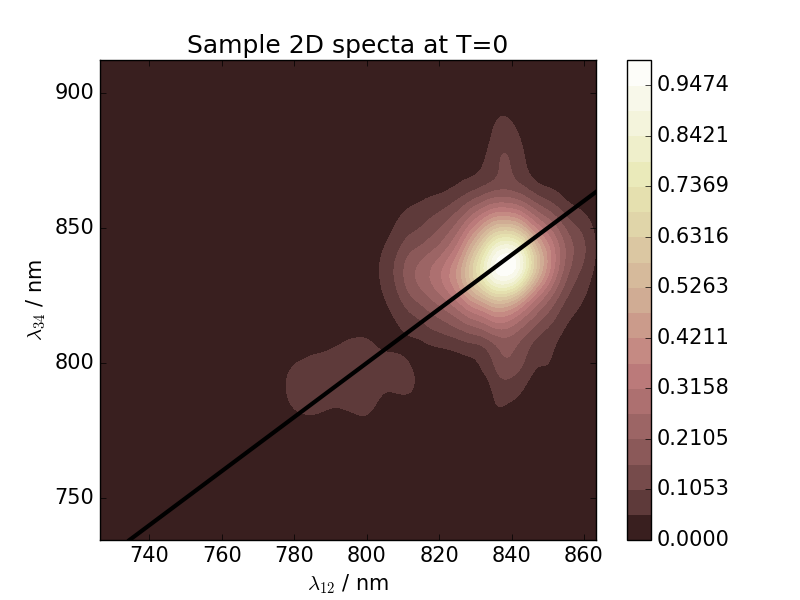
\includegraphics[width=1.0\columnwidth]{LH2_2DES_T0.png}
   \caption{This is data obtained from the Engel group for LH2.  Specifically this is the xzxz polarization setting at $T=0$.}
	\label{fig:LH2_2DES_T0}
\end{figure}

\begin{figure}
   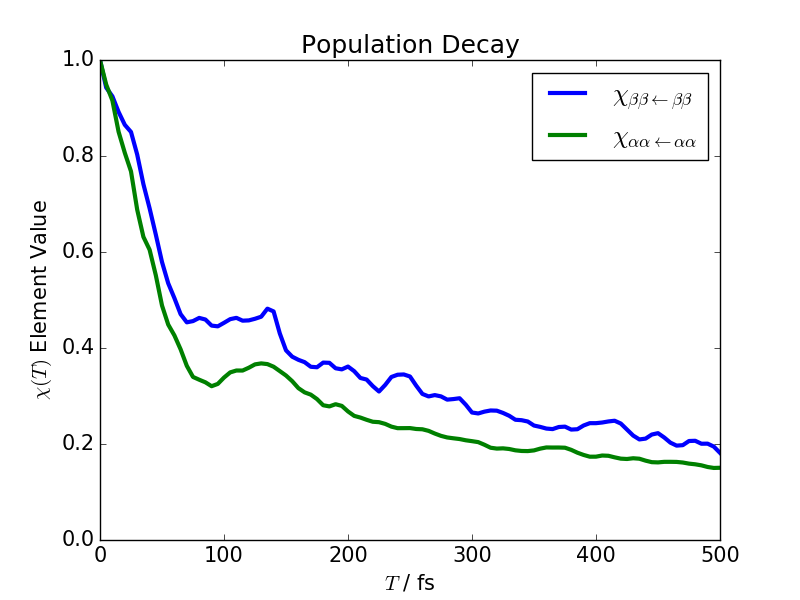
\includegraphics[width=1.0\columnwidth]{LH2_QPT_populationDecay.png}
   \caption{These are the two elements of the calculated Process Matrix which determine what proportion of the singly excited populations stay in the same state}
	\label{fig:LH2_QPT_populationDecay}
\end{figure}

\begin{figure}
   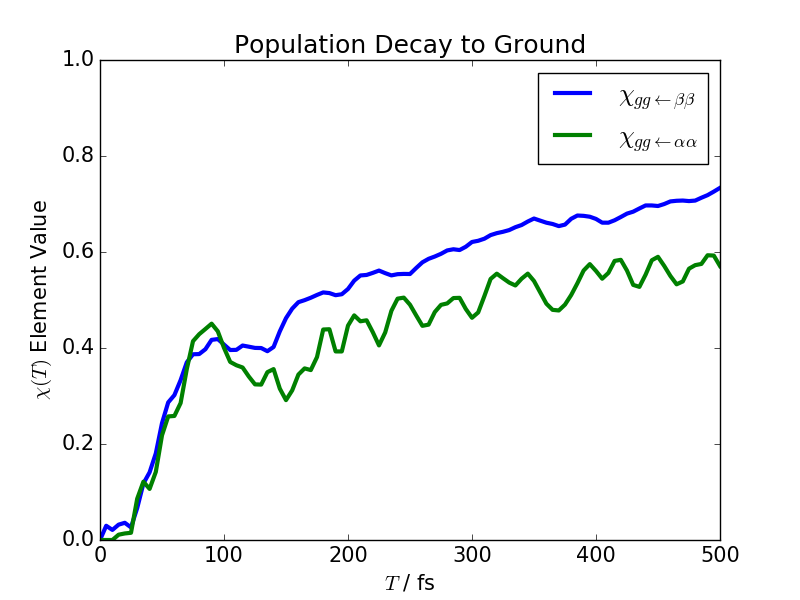
\includegraphics[width=1.0\columnwidth]{LH2_QPT_populationDecayToGround.png}
   \caption{These are the two elements of the calculated Process Matrix which determine the decay of the singly excited populations to the ground state population}
	\label{fig:LH2_QPT_populationDecayToGround}
\end{figure}

\begin{figure}
   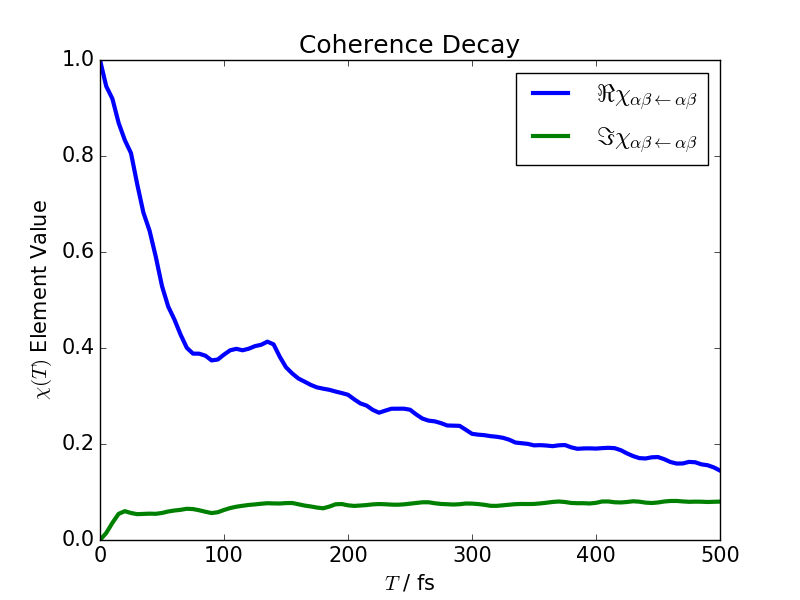
\includegraphics[width=1.0\columnwidth]{LH2_QPT_coherenceDecay.png}
   \caption{These are the two elements of the calculated Process Matrix which show what proportion of the singly excited coherences stay in the same coherent state}
	\label{fig:LH2_QPTcoherenceDecay}
\end{figure}

\begin{figure}
   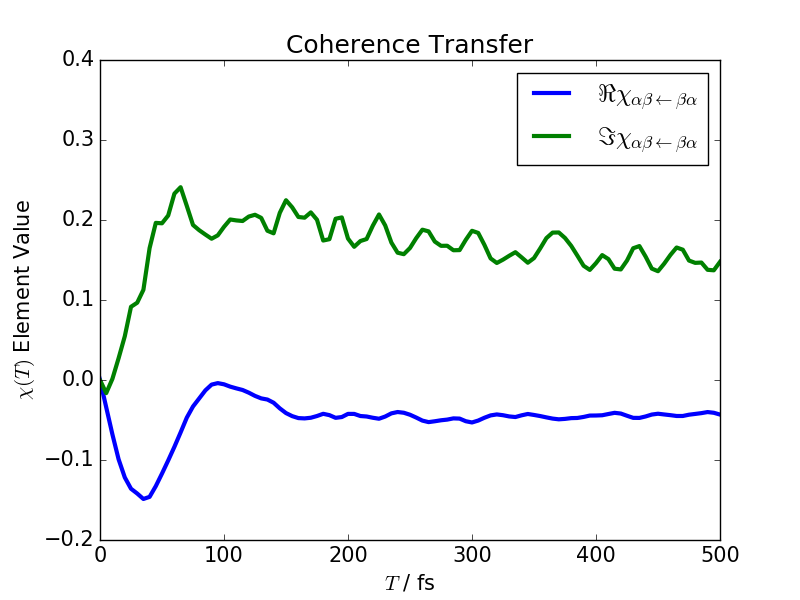
\includegraphics[width=1.0\columnwidth]{LH2_QPT_coherenceTransfer.png}
   \caption{These are the two elements of the calculated Process Matrix which determine what proportion of the singly excited coherences flop to the other coherence.}
	\label{fig:LH2_QPT_coherenceTransfer}
\end{figure}

\begin{figure}
   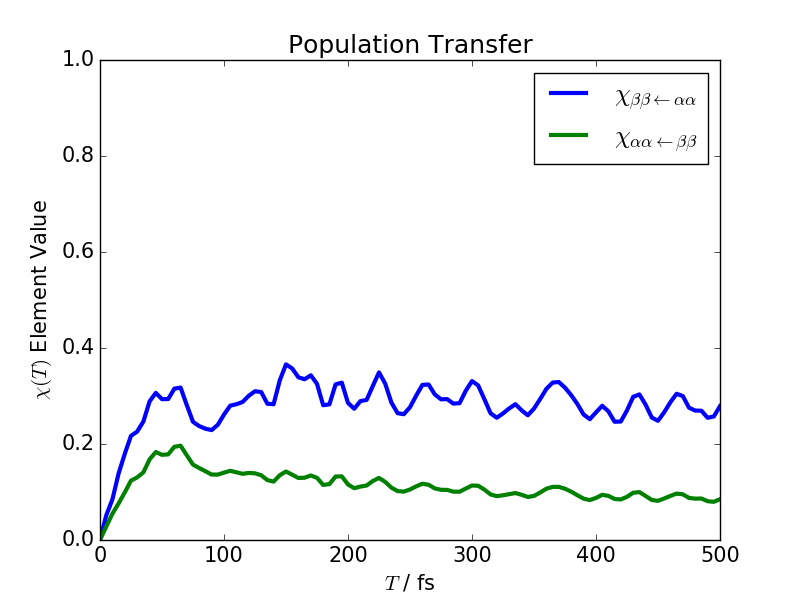
\includegraphics[width=1.0\columnwidth]{LH2_QPT_populationTransfer.png}
   \caption{These are the two elements of the calculated Process Matrix which determine the transfer of the singly excited populations  to the other singly excited population.  This is where we ran into problems.  The $\beta \beta$ population is higher in energy than the $\alpha \alpha$ population so if this graph was correct, there would be uphill energy transfer.}
	\label{fig:LH2_QPT_populationTransfer}
\end{figure}


Then lastly we have what turned out to be the problem element: the population transfer terms in Figure \ref{fig:LH2_QPT_populationTransfer}.  This figure indicates that there is a small, but insignificant uphill energy transfer.  Now this would be really cool if it were true as it would indicate that the bath imparted some useful energy to the light-harvesting apparatus of LH2.  But extraordinary claims require extraordinary evidence, so we need to revisit how we got here. to develop these Quantum Process Matrices, we had to assume that all three laser excitation pulses have the same power amplitude at both the $\alpha$ and $\beta$ transitions and at both polarizations.  This should not quite be true, and this assumption could very easily affect the expected probabilities of transfer into and out of $\alpha$ and $\beta$ states.  So we go back and see if we can correct this loose assumption.


\subsection{More Correct Forms for Laser Amplitude}

Knowing that we need to be more ignorant about the pulses, we recognize that for the $xzxz$ experiments, it is not reasonable to assume that all the beams are the same because they have different polarizations, we have to stop and go back a level of approximation.  We now assume that the x pulse amplitudes are the same and the z pulse amplitudes are the same
\begin{align*}
	\left \langle S_{\beta \alpha} \right \rangle^{xzxz} =&    -\frac{1}{10} B_1 A_2 B_1 a b  +  \frac{1}{15} B_1 B_2 A_1  b^2+ \frac{1}{30} B_1 B_2 A_1 a b  \\
	\left \langle S_{\beta \beta} \right \rangle^{xzxz} =&   -\frac{2}{15} B_1 B_2 B_1 b^2\\
	\left \langle S_{\alpha \alpha} \right \rangle^{xzxz} =& - \frac{2}{15} A_1 A_2 A_1 a^2  \\
	\left \langle S_{\alpha \beta} \right \rangle^{xzxz} =&   \frac{1}{15} A_1 A_2 B_1 a^2   + \frac{1}{30} A_1 A_2 B_1 a b -\frac{1}{10} A_1 B_2 A_1 a b
\end{align*}
and let's move things around to simplify them:
\begin{align*}
	\left \langle S_{\beta \alpha} \right \rangle^{xzxz} =&   B_1 A_2 B_1 \left(  -\frac{1}{10}  a b \right)   + B_1 B_2 A_1 \left(  \frac{1}{15}   b^2+ \frac{1}{30}  a b \right) \\
	\left \langle S_{\beta \beta} \right \rangle^{xzxz} =&  B_1 B_2 B_1 \left(  -\frac{2}{15}  b^2 \right) \\
	\left \langle S_{\alpha \alpha} \right \rangle^{xzxz} =& A_1 A_2 A_1\left( - \frac{2}{15}  a^2 \right)  \\
	\left \langle S_{\alpha \beta} \right \rangle^{xzxz} =&   A_1 A_2 B_1 \left( \frac{1}{15}  a^2   + \frac{1}{30}  a b \right)  + A_1 B_2 A_1  \left( -\frac{1}{10} a b   \right)
\end{align*}

Which should, in principle, be soluble with 8 equations and 8 unknowns.  For the 4 $zzzz$ equations, the solution is trivial.  When we put the four for $xzxz$ into Mathematica, both numerically and symbolically, it gives the null set.  What do we do?

\subsection{Ancilla}
We find that turning the equation into a quadratic with ancilla variables allows Mathematica to solve.  First some definitions
\begin{align*}
	\left \langle S_{\beta \alpha} \right \rangle^{xzxz} =&   B_1^2 A_2  \left(  -\frac{1}{10}  a b \right)   + A_1 B_1 B_2  \left(  \frac{1}{15}   b^2+ \frac{1}{30}  a b \right) \\
	\left \langle S_{\beta \beta} \right \rangle^{xzxz} =&  B_1^2 B_2  \left(  -\frac{2}{15}  b^2 \right) \\
	\left \langle S_{\alpha \alpha} \right \rangle^{xzxz} =& A_1^2 A_2  \left( - \frac{2}{15}  a^2 \right)  \\
	\left \langle S_{\alpha \beta} \right \rangle^{xzxz} =&   A_1 A_2 B_1 \left( \frac{1}{15}  a^2   + \frac{1}{30}  a b \right)  + A_1^2 B_2   \left( -\frac{1}{10} a b   \right)
\end{align*}
\begin{align}
	c_1 &= -\frac{a b}{10} \\
	c_2 &= \frac{b^2}{15} + \frac{a b}{30} \\
	c_3 &= \frac{-2 b^2}{15} \\
	c_4 &= \frac{-2 a^2}{15} \\
	c_5 &= \frac{a^2}{15} + \frac{a b}{30} \\
	c_6 &= \frac{-a b}{10}
\end{align}
now our ancilla variables:
\begin{align}
	q_1 &= B_1^2 \\
	q_2 &= B_1 B_2 \\
	q_3 &= A_1^2 \\
	q_4 &= A_1 A_2 \\
\end{align}
which turns the original system into:
\begin{align*}
	\left \langle S_{\beta \alpha} \right \rangle^{xzxz} =&   c_1  q_1 A_2  + c_2 q_2  A_1 \\
	\left \langle S_{\beta \beta} \right \rangle^{xzxz} =&   c_3 q_1 B_2  \\
	\left \langle S_{\alpha \alpha} \right \rangle^{xzxz} =&   c_4 q_3 A_2 \\
	\left \langle S_{\alpha \beta} \right \rangle^{xzxz} =&    c_5 q_4 B_1 +  c_6 q_3 B_2
\end{align*}
for Matlab fsolve, we need to turn into an equation which equals 0:
\begin{align}
	B_1^2 - q_1  \\
	B_1 B_2  - q_2 \\
	A_1^2 - q_3 \\
	A_1 A_2  - q_4 \\
	c_1 q_1 A_2+ c_2 q_2 A_1 - S_{ba}  \\
	c_3 q_1 B_2 - S_{bb} \\
	c_4 q_3 A_2 - S_{aa} \\
	c_5 q_4 B_1 + c_6 q_3 B_2 - S_{ab}
\end{align}
we also need to split into real and imaginary equations
\begin{align*}
	\real{B_1}^2 - \imag{B_1}^2 - \real{q_1}  \\
	2\real{B_1}\imag{B_1} - \imag{q_1}  \\
	\real{B_1}\real{ B_2} - \imag{B_1} \imag{B_2}  - \real{q_2} \\
	\real{B_1}\imag{ B_2} + \imag{B_1} \real{B_2}  - \imag{q_2} \\
	\real{A_1}^2 - \imag{A_1}^2 - \real{q_3} \\
	2 \real{A_1}\imag{A_1} - \imag{q_3} \\
	\real{A_1}\real{ A_2} - \imag{A_1} \imag{A_2}  - \real{q_4} \\
	\real{A_1}\imag{ A_2} + \imag{A_1} \real{A_2}  - \imag{q_4} \\
	c_1 \left( \real{q_1} \real{A_2} - \imag{q_1} \imag{A_2}  \right) + c_2 \left( \real{q_2} \real{A_1} - \imag{q_2} \imag{A_1}  - \real{S_{ba}} \right) \\
	c_1 \left( \real{q_1} \imag{A_2} + \imag{q_1} \real{A_2}  \right) + c_2 \left( \real{q_2} \imag{A_1} + \imag{q_2} \real{A_1}  - \imag{S_{ba}} \right) \\
	c_3 \left( \real{q_1} \real{B_2} - \imag{q_1} \imag{B_2}  \right) - \real{S_{bb}} \\
	c_3 \left( \real{q_1} \imag{B_2} + \imag{q_1} \real{B_2}  \right) - \imag{S_{bb}} \\
	c_4 \left( \real{q_3} \real{A_2} - \imag{q_3} \imag{A_2}  \right) - \real{S_{aa}} \\
	c_4 \left( \real{q_3} \imag{A_2} + \imag{q_3} \real{A_2}  \right) - \imag{S_{aa}} \\
	c_5 \left( \real{q_4} \real{B_1} - \imag{q_4} \imag{B_1}  \right) + c_6 \left( \real{q_3} \real{B_2} - \imag{q_3} \imag{B_2}  - \real{S_{ab}} \right) \\
	c_5 \left( \real{q_4} \imag{B_1} + \imag{q_4} \real{B_1}  \right) + c_6 \left( \real{q_3} \imag{B_2} + \imag{q_3} \real{B_2}  - \imag{S_{ab}} \right)
\end{align*}
but this strategy does not yield answers in fsolve.

\subsection{Experimental Considerations}

Perhaps by considering the experimental setup, we can eliminate variables and make the equations solvable.  The Engel group tells us they generate an x polarization by putting a half waveplate in front of the beam.  They use a different waveplate for the first and third pulse, unfortunately, but for now we are going to assume they both impart a perfect, identical phase-shift and  contemplate how this additional information changes the equations.

Half waveplates are designed to import a $\pi$ phase-shift.  The amplitude effect of this is $e^{i \pi} = -1$.  This means that $A_1 = -A_2$ and the same for $B$.  We turns these constants into just A and B.

\begin{align*}
	\left \langle S_{\beta \alpha} \right \rangle^{xzxz} =&    -\frac{1}{10} B^2 (-A)  a b  +  \frac{1}{15} B (- B) A  b^2+ \frac{1}{30} B (- B) A a b  \\
	\left \langle S_{\beta \beta} \right \rangle^{xzxz} =&   -\frac{2}{15} B (- B) B b^2\\
	\left \langle S_{\alpha \alpha} \right \rangle^{xzxz} =& - \frac{2}{15} A (-A) A a^2  \\
	\left \langle S_{\alpha \beta} \right \rangle^{xzxz} =&   \frac{1}{15} A (-A) B a^2   + \frac{1}{30} A (-A) B a b -\frac{1}{10} A (-B) A a b
\end{align*}
which simplifies to
\begin{align*}
	\left \langle S_{\beta \alpha} \right \rangle^{xzxz} =&    \frac{1}{10} B^2 A  a b  -  \frac{1}{15} B^2A  b^2 - \frac{1}{30} B^2 A a b  \\
	\left \langle S_{\beta \beta} \right \rangle^{xzxz} =&   \frac{2}{15} B^3 b^2\\
	\left \langle S_{\alpha \alpha} \right \rangle^{xzxz} =& \frac{2}{15} A^3  a^2  \\
	\left \langle S_{\alpha \beta} \right \rangle^{xzxz} =&   -\frac{1}{15} A^2 B a^2   - \frac{1}{30} A^2 B a b + \frac{1}{10} A^2 B a b
\end{align*}
and further simplifies to
\begin{align*}
	\left \langle S_{\beta \alpha} \right \rangle^{xzxz} =&   B^2 A \left( \frac{1}{10}   a b  -  \frac{1}{15}   b^2 - \frac{1}{30}  a b \right) \\
	\left \langle S_{\beta \beta} \right \rangle^{xzxz} =&   \frac{2}{15} B^3 b^2\\
	\left \langle S_{\alpha \alpha} \right \rangle^{xzxz} =& \frac{2}{15} A^3  a^2  \\
	\left \langle S_{\alpha \beta} \right \rangle^{xzxz} =& A^2 B \left(  -\frac{1}{15}  a^2   - \frac{1}{30} a b + \frac{1}{10}  a b   \right)
\end{align*}
and again to
\begin{align*}
	\left \langle S_{\beta \alpha} \right \rangle^{xzxz} =&   B^2 A \left( \frac{1}{15}   a b  -  \frac{1}{15}   b^2 \right) \\
	\left \langle S_{\beta \beta} \right \rangle^{xzxz} =&   \frac{2}{15} B^3 b^2\\
	\left \langle S_{\alpha \alpha} \right \rangle^{xzxz} =& \frac{2}{15} A^3  a^2  \\
	\left \langle S_{\alpha \beta} \right \rangle^{xzxz} =& A^2 B \left(\frac{1}{15}  a b   -\frac{1}{15}  a^2    \right)
\end{align*}
and again to
\begin{align*}
	\left \langle S_{\beta \alpha} \right \rangle^{xzxz} =&   B^2 A \frac{1}{15}  \left(    a b  -  b^2 \right) \\
	\left \langle S_{\beta \beta} \right \rangle^{xzxz} =&   \frac{2}{15} B^3 b^2\\
	\left \langle S_{\alpha \alpha} \right \rangle^{xzxz} =& \frac{2}{15} A^3  a^2  \\
	\left \langle S_{\alpha \beta} \right \rangle^{xzxz} =& A^2 B \frac{1}{15}  \left( a b   - a^2    \right)
\end{align*}
But this method did not yield a solution either.


\subsection{Conclusion}
While we thought that we could get out a process matrix for data given to us by the Engel group, and we did get one that had some radical claims in it with equally dubious assumptions behind them, we found no way to de-dubify the assumptions and thus we left it at this.









\section{Investigating Conical Intersections Using Pulse-width Dependent Dynamics}
A very simple molecular Hamiltonian looks like this:
\begin{align*}
	\hat{H} &= \frac{1}{2 \mu} \nabla^2_{R} + \frac{1}{2 m_e} \nabla^2_{r}  +  \frac{Z_1 Z_2}{R^2} + \frac{Z_1}{r_1^2} + \frac{Z_2}{r_2^2}
\end{align*}
Which we can separate into a nuclear kinetic, an electronic kinetic, a nuclear potential and an electron-nuclear potential:
\begin{align*}
	\hat{H} &= T_n + T_e  + V_n(R) + V_e (R)  +  V_{en} (R, r)
\end{align*}
If we assume we can separate the components which solve the wavefunction into an electronic and a nuclear part:
\begin{align*}
	\Psi(R, r) = \psi(R) \phi(r)
\end{align*}
which is the heart of the Born-Oppenheimer approximation.  But it's not terribly physical.  This approximation, effectively, says that even if you compress the bond in, say, a hydrogen molecule, to some fraction of the equilibrium length, the electronic configuration would be the same.  Which is clearly not true.   As the nuclei move, you would of course expect the oppositely charged electrons to ``follow'' them around.

So the next level of approximation down is to say that the nuclei will still probably not see the electrons moving around, the electrons will definitely see the nuclei if they change positions and because the electrons move around much faster, than the nuclei, it would make sense that we would see them react to a change in position of the nuclei.  So we change the prototype wavefunction to have a nuclear part and an electronic part, conditioned on the nuclear coordinates:
\begin{align*}
	\Psi(R, r) = \psi(R) \phi(r;R)
\end{align*}
You can imagine this will complicate things but still allow us more simplicity and tractability than would be had through not separating things at all.  For example, this gives us the ability to solve the electronic part of the equation for every possible nuclear configuration $R$ to come up with an electronic energy landscape:
\begin{align*}
	\hat{H}_e\phi(r;R) &= ( T_e  + V_e (R)  +  V_{en} (R, r) )\phi(r;R) = E(R) \phi(r;R)
\end{align*}
where it's important here to recognize we are able to solve for the full electronic spectrum
\begin{align*}
	\hat{H}_e\phi(r;R) = \hat{H}_e\sum_{n}a_n \phi_n(r;R)  = \phi(r;R) = \sum_{n} E_n(R) a_n \phi_n(r;R)
\end{align*}
But that's not the whole equation is it?  We can take this solution to the electronic equation and put it back into the full equation:
\begin{align*}
	\hat{H}\left[ \psi(R) \phi(r;R) \right] &= \left(  T_n + T_e  + V_n(R) + V_e (R)  +  V_{en} (R, r) \right)\left[ \psi(R) \phi(r;R) \right] \\
	&= \left( T_e + V_e (R)  +  V_{en} (R, r) \right)\left[ \psi(R) \phi(r;R) \right] + \left(  T_n + V_n(R) \right)\left[ \psi(R) \phi(r;R) \right]
\end{align*}
none of the operators in the front will change the nuclear part of the wavefunction in any manner so that we can just substitute in the solution to the electronic problem: $E(R)$.  It seems a natural pairing to go with $V_N(R)$ so we do that
\begin{align*}
	\hat{H}\left[ \psi(R) \phi(r;R) \right] &= \left( E(R) + V_n(R)  \right)\left[ \psi(R) \phi(r;R) \right] + T_n \left[ \psi(R) \phi(r;R) \right]
\end{align*}
and are left with one term.  Which is going to cause some problems.  This is because it will introduce new terms as the nuclear kinetic operator acts on the electronic wavefunction also,
\begin{align*}
	T_n \Psi(R, r) &=\frac{1}{2 \mu} \nabla^2_{R}  \psi(R) \phi(r;R) \\
	&=\frac{1}{2 \mu} \nabla_{R} \cdot \left(    \psi(R) \nabla_{R}  \phi(r;R) + \nabla_{R}  \psi(R) \phi(r;R) \right) \\
	&=\frac{1}{2 \mu}  \left(    \psi(R) \nabla_{R}^2 \phi(r;R)  +  \nabla_{R}  \psi(R) \cdot  \nabla_{R}  \phi(r;R) + \nabla_{R}^2  \psi(R) \phi(r;R)  + \nabla_{R}  \psi(R) \cdot \nabla_{R} \phi(r;R) \right) \\
	&=\frac{1}{2 \mu}  \left(    \psi(R) \nabla_{R}^2 \phi(r;R)  + 2  \nabla_{R}  \psi(R) \cdot  \nabla_{R}  \phi(r;R) \right)  + \frac{1}{2 \mu} \nabla_{R}^2  \psi(R) \phi(r;R)
\end{align*}

The third term is the boring old nuclear kinetic energy we know about from the Born-Oppenheimer approximation wavefunction, but the first two terms complicate things and they are the heart of why we are talking here.  If we decide to ignore then:
\begin{align*}
	\hat{H}\left[ \psi(R) \phi(r;R) \right] &= \left( E(R) + V_n(R)  \right)\left[ \psi(R) \phi(r;R) \right] +\phi(r;R)  T_n  \psi(R)  \\
	&= \phi(r;R)  \left( E(R) + V_n(R)  + T_n \right) \psi(R) \\
	\hat{H} \psi(R)  &=  \left( E(R) + V_n(R)  + T_n \right) \psi(R)
\end{align*}
we can basically prescribe that you go solve the electronic problem $E(R)$ and then come back to solve the nuclear problem.  The solutions to this problem are called the ``\textbf{Adiabatic Representation}'' and represent the solutions which preserve ordering of the energy levels so for the energy eigenstates of the problem, $\Psi_i (R, r) = \psi_i(R) \phi_i(r;R) $ the set of $E_i$'s form a ladder of energies, going up from 0 to infinity.

Now let's look at what happens when we put those exact adiabatic solutions into the full Hamiltonian:
\begin{align}
	\hat{H} \Psi_i(R,r) &=    \phi_i(r;R) \left( E(R) + V_n(R)  + T_n \right)\psi_i(R) + \frac{1}{2 \mu}  \left(    \psi_i(R) \nabla_{R}^2 \phi_i(r;R)  + 2  \nabla_{R}  \psi_i(R) \cdot  \nabla_{R}  \phi_i(r;R) \right)
\end{align}
and let's average away the electronic degrees of freedom by coming in with $\phi_j(r;R)$ and integrating out the electronic degrees of freedom:
\begin{align}
	\int dr \phi_j(r;R) \hat{H} \Psi_i(R,r) = H_{i j}(R) \psi_i(R)  &=   \int dr \psi_j(R) \phi_j(r;R) \phi_i(r;R) \left( E(R) + V_n(R)  + T_n \right)\psi_i(R) \\
	&+  \int dr  \phi_j(r;R)  \frac{1}{2 \mu}  \left(    \psi_i(R) \nabla_{R}^2 \phi_i(r;R)  + 2  \nabla_{R}  \psi_i(R) \cdot  \nabla_{R}  \phi_i(r;R) \right)  \\
	&=   \delta_{ij}  \left( E(R) + V_n(R)  + T_n \right)\psi_i(R) \\
	&+   \frac{1}{2 \mu}  \left[ \int dr \phi_j(r;R)  \nabla_{R}^2 \phi_i(r;R)   \right] \psi_i(R)\\
	&+ \frac{1}{ \mu} \left[ \int dr \phi_j(r;R)  \nabla_{R}  \phi_i(r;R)   \right] \cdot \nabla_{R}  \psi_i(R)
\end{align}
So we have additional quantities to calculate from the electronic states:
\begin{align}
	\vec{T}^{(1)}_{ij}(R) &= \frac{1}{ \mu} \left[ \int dr \phi_j(r;R)  \nabla_{R}  \phi_i(r;R)   \right] \\
	T^{(2)}_{ij}(R) &=  \frac{1}{2 \mu}  \left[ \int dr \phi_j(r;R)  \nabla_{R}^2 \phi_i(r;R)   \right]
\end{align}
Which when all is said and done, we are left with a final answer of:
\begin{align}
	 H_{i j}(R) \psi_i(R)&=   \delta_{ij}  \left( E(R) + V_n(R)  + T_n \right)\psi_i(R) + T^{(2)}_{ij}(R)  \psi_i(R) +\vec{T}^{(1)}_{ij}(R)  \cdot \nabla_{R}  \psi_i(R) \\
	 &=  \left[  \delta_{ij}  \left( E(R) + V_n(R)  + T_n \right)  +\vec{T}^{(1)}_{ij}(R)  \cdot \nabla_{R}  + T^{(2)}_{ij}(R)  \right]\psi_i(R)
\end{align}
We can prove that
\begin{align}
	\text{Re} [\vec{T}^{(1)}_{ij}(R) ] &= 0 \\
	\vec{T}^{(1)}_{aa}(R) &= 0
\end{align}
\subsection{Adiabatic Representation}
Say we don't care about energy ordering, and we only care about the electronic character of the wavefunctions staying the same.   We can instead pick some arbitrary geometry--let's call it $R_0$--and then solve the full Hamiltonian for each of those geometries:
\begin{align}
	\Psi(R, r) = \sum_i \phi_i(r;R_0) \psi_i^{(0)}(R)
\end{align}
And now let's do what we did last time and act the Hamiltonian on the electronic part of the wavefunction:
\begin{align*}
	\hat{H} \phi_i(r;R_0) &= \left(  T_n + T_e  + V_n(R) + V_e (r)  +  V_{en} (R, r) \right)\phi_i(r;R_0) \\
	&= \left(  T_e  + V(r, R_0) \right)\phi_i(r;R_0) = E_i (R_0)\phi_i(r;R_0)
\end{align*}
and that will be the equation we solve to get the electronic states.  We can then put the whole thing with the vibrational part back in
\begin{align*}
	\hat{H} \phi_i(r;R_0) \psi_i^{(0)}(R) &= \left(  T_n + T_e  + V_n(R) + V_e (r)  +  V_{en} (R, r) \right)\phi_i(r;R_0) \psi_i^{(0)}(R) \\
	&= \left(   T_e + V (R, r)  + T_n  \right)\phi_i(r;R_0) \psi_i^{(0)}(R) \\
	&= \left(   T_e + V (R, r)  + V (R_0, r)  - V (R_0, r)  + T_n  \right)\phi_i(r;R_0) \psi_i^{(0)}(R) \\
	&= \left(   T_e + V (R_0, r)    \right)\phi_i(r;R_0) \psi_i^{(0)}(R)  + \left(   T_n  + V (R, r)  - V (R_0, r)  \right)\phi_i(r;R_0) \psi_i^{(0)}(R) \\
	&= E_i(R_0) \phi_i(r;R_0) \psi_i^{(0)}(R)  + \left(   T_n  + V (R, r)  - V (R_0, r)  \right)\phi_i(r;R_0) \psi_i^{(0)}(R)
\end{align*}
Now we come in with the $j$th basis function and integrate out over the electronic degrees of freedom\begin{align*}
	\hat{H}_{ij}  \psi_i^{(0)}(R) &= \int dr \phi_j(r;R_0) E_i(R_0) \phi_i(r;R_0) \psi_i^{(0)}(R)  \\
	&+\int dr \phi_j(r;R_0) \left(   T_n  + V (R, r)  - V (R_0, r)  \right)\phi_i(r;R_0) \psi_i^{(0)}(R)  \\
	&= \delta_{ij} E_i(R_0) \psi_i^{(0)}(R) + \delta_{ij} T_n  \psi_i^{(0)}(R)   + \int dr \phi_j(r;R_0) \left(  V (R, r)  - V (R_0, r)  \right)\phi_i(r;R_0) \psi_i^{(0)}(R) \\
	&= \delta_{ij} \left[ E_i(R_0) + T_n  \right] \psi_i^{(0)}(R)   + U_{ji}(R) \psi_i^{(0)}(R) \\
	 U_{ji}(R) &= \int dr \phi_j(r;R_0) \left(  V (R, r)  - V (R_0, r)  \right)\phi_i(r;R_0)
\end{align*}

\subsection{Detecting A Conical Intersection}
Looking at the diabatic energy corrections, one finds a term in the Hamiltonian which looks like this:
\begin{align}
   2\nabla_R \psi(R) \cdot \nabla_R \phi(r;R)
\end{align}
the second part of which can be integrated out to find a vector-like coupling between two different electronic states and the first part of which is clearly the nuclear momentum.  This ends up giving a term in the Hamiltonian proportional to:
\begin{align}
   \vec{p}_{r}\cdot \vec{J}_{i,j}
\end{align}


So why not manipulate the momentum of the wavefunction to manipulate the dynamics and thus create a way of detecting a electronic vector coupling $\vec{J}_{i,j}$.  Preliminary work on this proved not to be fruitful.  I wasn't, however, entirely sure what I was looking for and would return to this hypothesis again if I ever think that I have found something that might actually be different.  By including this in my thesis, even though no one will read it, I hope to possibly inspire someone to continue this work.
